\documentclass{article}
% if you need to pass options to natbib, use, e.g.:
%     \PassOptionsToPackage{numbers, compress}{natbib}
% before loading neurips_2024

% ready for submission
\usepackage[final]{neurips_2024}
% to compile a preprint version, e.g., for submission to arXiv, add add the
% [preprint] option:
%     \usepackage[preprint]{neurips_2024}

% to compile a camera-ready version, add the [final] option, e.g.:
%     \usepackage[final]{neurips_2024}

% to avoid loading the natbib package, add option nonatbib:
% \usepackage[nonatbib]{neurips_2024}

\usepackage[utf8]{inputenc} % allow utf-8 input
\usepackage[T1]{fontenc}    % use 8-bit T1 fonts
\usepackage{hyperref}       % hyperlinks
\usepackage{url}            % simple URL typesetting
\usepackage{booktabs}       % professional-quality tables
\usepackage{amsfonts}       % blackboard math symbols
\usepackage{nicefrac}       % compact symbols for 1/2, etc.
\usepackage{microtype}      % microtypography
\usepackage{xcolor}         % colors
\usepackage{amsmath}
\usepackage{adjustbox}
\usepackage{array}
\usepackage{xcolor,colortbl}
\usepackage{algorithm}
\usepackage{algpseudocode}
\usepackage{multicol}
\usepackage{caption}
\usepackage{graphicx}
\usepackage{subcaption}
\usepackage{wrapfig}
\DeclareMathOperator*{\argmin}{arg\,min}
\DeclareMathOperator*{\argmax}{arg\,max}
\newtheorem{theorem}{Theorem}
\renewcommand{\algorithmicensure}{\textbf{Initialize:}}

\newcolumntype{R}[2]{%
    >{\adjustbox{angle=#1,lap=\width-(#2)}\bgroup}%
    l%
    <{\egroup}%
}
\newcommand*\rot{\multicolumn{1}{R{45}{0em}}}
\newcommand{\fig}[1]{\textbf{\color{blue}Fig: #1}}
\newcommand{\tab}[1]{\textbf{\color{red}Tab: #1}}
\newenvironment{Figure}
  {\par\medskip\noindent\minipage{\linewidth}}
  {\endminipage\par\medskip}
\definecolor{lightgrey}{rgb}{0.95, 0.95, 0.95}
\definecolor{softblue}{rgb}{0.22, 0.59, 1.00}
\definecolor{softorange}{rgb}{1.00, 0.52, 0.00}
\definecolor{softgreen}{rgb}{0.45, 0.62, 0.5}

\title{Advancing Cross-domain Discriminability in Continual Learning of Vision-Language Models}

% The \author macro works with any number of authors. There are two commands
% used to separate the names and addresses of multiple authors: \And and \AND.
%
% Using \And between authors leaves it to LaTeX to determine where to break the
% lines. Using \AND forces a line break at that point. So, if LaTeX puts 3 of 4
% authors names on the first line, and the last on the second line, try using
% \AND instead of \And before the third author name.

\author{
  Yicheng Xu$^{1}$\thanks{Equal contribution}\ \ \ \ Yuxin Chen$^{2}$\footnotemark[1]\ \ \ \ Jiahao Nie$^{3}$\ \ \ \ \\ 
  \textbf{Yusong Wang}$^{1}$\ \ \ \ \textbf{Huiping Zhuang}$^{4, 5}$\thanks{Corresponding author: hpzhuang@scut.edu.cn}\ \ \ \ \textbf{Manabu Okumura}$^{1}$ \smallskip\\
  $^{1}$Institute of Science Tokyo\ \ \ \ $^{2}$University of California Berkeley\\ $^{3}$Nanyang Technological University\ \ \ \ $^{4}$South China University of Technology\\
  $^{5}$Greater Bay Area Institute for Innovation, Hunan University, China \smallskip\\
  \texttt{yxu040@e.ntu.edu.sg, yuxinc@berkeley.edu}
}


\begin{document}

\maketitle
% \def\thefootnote{*}\footnotetext{Equal Contribution}


\begin{abstract}
Continual learning (CL) with Vision-Language Models (VLMs) has overcome the constraints of traditional CL, which only focuses on previously encountered classes. During the CL of VLMs, we need not only to prevent the catastrophic forgetting on incrementally learned knowledge but also to preserve the zero-shot ability of VLMs. However, existing methods require additional reference datasets to maintain such zero-shot ability and rely on domain-identity hints to classify images across different domains. In this study, we propose \textbf{R}egression-based \textbf{A}nalytic \textbf{I}ncremental \textbf{L}earning (RAIL), which utilizes a recursive ridge regression-based adapter to learn from a sequence of domains in a non-forgetting manner and decouple the cross-domain correlations by projecting features to a higher-dimensional space. Cooperating with a training-free fusion module, RAIL absolutely preserves the VLM's zero-shot ability on unseen domains without any reference data.
Additionally, we introduce \textbf{Cross}-domain \textbf{T}ask-\textbf{A}gnostic \textbf{I}ncremental \textbf{L}earning (X-TAIL) setting. In this setting, a CL learner is required to incrementally learn from multiple domains and classify test images from both seen and unseen domains without any domain-identity hint.
We theoretically prove RAIL's absolute memorization on incrementally learned domains. Experiment results affirm RAIL's state-of-the-art performance in both X-TAIL and existing Multi-domain Task-Incremental Learning settings. The code is released at \url{https://github.com/linghan1997/Regression-based-Analytic-Incremental-Learning}.
\end{abstract}

\section{Introduction}
\label{sec:intro}
Continual learning (CL)~\cite{hadsell2020embracing, de2021continual, wang2024comprehensive} is a crucial area in machine learning, which requires a learner to incrementally learn new data instead of training from scratch. The main challenge in CL is known as catastrophic forgetting~\cite{mccloskey1989catastrophic}, where learning new knowledge results in the forgetting of the old one. To this end, various CL approaches~\cite{kirkpatrick2017overcoming, li2017learning, rebuffi2017icarl, buzzega2020dark, wang2024comprehensive, liu2024locality} have been proposed to solve the forgetting issue. As a typical CL setting, Class-Incremental Learning (CIL) (Fig.~\ref{fig:xtail} (a)) aims to achieve robust discriminability on all seen classes. Despite the advancements, existing approaches mainly focus on classifying images only from seen classes, thereby limiting the model's generalizability.

Consequently, Zheng \textit{et al.}~\cite{Zheng_2023_ICCV} proposed Multi-domain Task-Incremental Learning (MTIL), which cooperates CL with the zero-shot ability of Vision-Language Models (VLMs)~\cite{li2021align,kim2021vilt,radford2021learning,li2022blip} such as CLIP~\cite{radford2021learning}. This integration equips models with the ability to classify domains they have not yet encountered, enhancing their generalizability across multiple domains (Fig.~\ref{fig:xtail} (b)). Several methods~\cite{Zheng_2023_ICCV, yu2024boosting} have been specifically designed for MTIL, in which the model is required to retain both the incrementally learned knowledge during CL and the zero-shot ability of VLMs. However, these methods require a domain-identity hint to indicate the specific domain of the test image, which is often not applicable in real-world scenarios~\cite{rebuffi2017icarl}. Additionally, the use of reference datasets during training is necessary to maintain pre-trained VLMs' zero-shot performance.


% \rv{Continual learning (CL)~\cite{hadsell2020embracing, de2021continual, wang2024comprehensive} is a crutial area in machine learning. It focuses on developing methods that help models incrementally acquire new knowledge while addressing the issue of catastrophic forgetting~\cite{mccloskey1989catastrophic}. 
% % This is essential for practical applications where input data continuously evolves, such as in robotics and real-time data processing systems~\cite{churamani2020continual, li2019rilod}.
% Despite the advancements, existing CL approaches~\cite{kirkpatrick2017overcoming, li2017learning, rebuffi2017icarl, buzzega2020dark, wang2024comprehensive} mainly focus on classification with a limited and incrementally accumulated label, which restricts the model's capabilities, particularly in the early steps of continual learning.}

% With the emergence of Vision-Language Models (VLMs)~\cite{li2021align,kim2021vilt,radford2021learning,li2022blip} such as CLIP~\cite{radford2021learning}, the nature of Open Vocabulary~\cite{wu2024towards} allows models to classify classes not explicitly defined during training. Leveraging this ability, several studies~\cite{Zheng_2023_ICCV, yu2024boosting} propose using a pre-trained CLIP to incrementally learn from training data in new domains while maintaining the zero-shot ability to classify unseen classes. However, these approaches commonly require a domain-identity hint to indicate the specific domain of the test image, a challenging requirement that represents a strong assumption often not applicable in real-world scenarios~\cite{rebuffi2017icarl}.

To address the aforementioned limitations, we introduce \textbf{R}egression-based \textbf{A}nalytic \textbf{I}ncremental \textbf{L}earning (RAIL), a novel approach that incrementally learns new knowledge and performs effectively on both seen and unseen domains. Specifically, we leverage non-linear projection functions from both primal and dual perspectives to enhance the expressiveness of features extracted by the pre-trained CLIP. It endows the learner with the ability to classify images in a cross-domain label set without any domain-identity hint. In the incremental learning process, RAIL utilizes a ridge regression-based adapter that updates the parameters recursively. This is identical to learning on all encountered domains at once, achieving absolute memorization on learned domains. Additionally, we freeze the pre-trained CLIP and design a training-free fusion module to determine whether the test data belongs to seen or unseen domains. This strategy absolutely preserves CLIP's zero-shot ability on unseen domains, meeting practical requirements for models deployed in dynamic environments.

To demonstrate the effectiveness of our method, we propose \textbf{Cross}-domain \textbf{T}ask-\textbf{A}gnostic \textbf{I}ncremental \textbf{L}earning (X-TAIL) setting as illustrated in Fig.~\ref{fig:xtail} (c). Particularly, X-TAIL requires CL methods to incrementally transfer a pre-trained VLM to multiple domains while evaluating the model's performance on both seen and unseen domains. Moreover, domain hints are forbidden in X-TAIL, making it more realistic and challenging~\cite{wang2024comprehensive}. As a result, effective CL methods must classify a test image into the correct domain and class simultaneously.

\begin{figure}[t]
    \centering
    \includegraphics[width=\linewidth]{Figures/X-TAIL.pdf}
    \caption{\textbf{Comparison of different CL settings.}
    (a) In CIL, models classify images within all previously encountered classes. (b) In MTIL, models classify images from both seen and unseen domains based on the given domain-identities. (c) In X-TAIL, models classify images from both seen and unseen domains without any  domain-identity hint.}
    \vspace{-3mm}
    \label{fig:xtail}
\end{figure}

% Our RAIL demonstrates its absolute non-forgetting advantage in both zero-shot transfer ability and incremental learning ability. It achieves state-of-the-art performances on our X-TAIL as well as on existing Multi-domain Task-Incremental Learning (MTIL)~\cite{Zheng_2023_ICCV} settings.

Our contributions are summarized as follows:
\begin{itemize}
    \item We propose a new CL method RAIL to incrementally adapt the pre-trained VLM to multiple domains without forgetting both pre-trained and incrementally learned knowledge.
    \item To meet the practical scenario where CL methods need to sequentially learn data from new domains and classify images across these domains, we propose a new setting X-TAIL to evaluate the preservation of VLM's zero-shot ability and the adaptability to new domains.
    \item We theoretically prove the RAIL's absolute memorization on incrementally learned domains and demonstrate that the zero-shot ability of the pre-trained VLM on unseen domains is absolutely preserved.
    \item We empirically show that the proposed method achieves state-of-the-art performances on both existing MTIL and the novel X-TAIL settings.
\end{itemize}

\section{Related work}
\label{sec:related_work}
% \subsection{Continual learning}
Early CL methods focused on Task-Incremental Learning (TIL)~\cite{hsu2018re}, where a task-id is given during testing. Subsequently, a more practical and challenging setting of Class-Incremental Learning (CIL)~\cite{rebuffi2017icarl} was proposed, where the access to the task-id is forbidden at inference time. Methods for CIL must therefore distinguish between all classes encountered in learned tasks.
More recently, Zheng \textit{et al.}~\cite{Zheng_2023_ICCV} proposed Multi-Domain Task-Incremental Learning (MTIL), which is especially designed to evaluate CL methods with pre-trained VLMs. In MTIL, a pre-trained VLM continually adapts to multi-domain tasks. The performance on both seen and unseen tasks measure the retention of both incrementally acquired and pre-trained knowledge. However, it still requires the task-id to create specific domain label space at inference time.
Apart from them, X-TAIL combines the challenges of both CIL and MTIL, in which the model learns new classes from various incoming domains and distinguishes between both seen and unseen classes without any domain-identity.

Prevailing continual learning methods include replay-based, distillation-based, regularization-based, and architecture-based approaches~\cite{wang2024comprehensive}. Replay-based methods such as iCaRL \cite{rebuffi2017icarl} typically store a small portion of the previous task data as exemplars. The model is then trained jointly on new task data and the saved exemplars to preserve the previous knowledge. Distillation-based methods such as LwF \cite{li2017learning} use either weight or function regularization to transfer knowledge from the previous model to the current model for knowledge distillation. Regularization-based methods such as ZSCL~\cite{Zheng_2023_ICCV} penalize the shift of either model parameter or feature space by adding a regularization term to the cross-entropy loss function. To preserve the robustness of the strong pre-trained model without access to the pre-trained dataset, ZSCL utilizes large-scale reference datasets to regularize the parameter space. 
Architecture-based methods~\cite{mallya2018piggyback, wang2022s, wang2024hierarchical} expand the model by constructing task-specific parameters to avoid inter-task interference. For example, MoE-Adapters~\cite{yu2024boosting} cooperates the pre-trained CLIP with mixture of experts (MoE)~\cite{jacobs1991adaptive} to learn from different domains. By leveraging a reference dataset to initialize a task-id indicator, it enables the model to distinguish unseen tasks from seen ones.

The aforementioned methods either neglect the forgetting issue of pre-trained knowledge or require multiple iterations and large-scale reference datasets for training, making it challenging to efficiently adapt to new data in continual learning scenarios. By contrast, RAIL employs an analytical solution that achieves the optimum in a single epoch without additional reference data, ensuring its efficiency.

% \subsection{Domain transfer with VLMs}
% Pre-trained on large vision-text datasets, VLMs have achieved remarkable performance on various downstream vision tasks. The pre-trained VLMs have been utilized by various methods \cite{gao2024clip} \cite{zhang2021tip} \cite{Zhou_2022} \cite{zhou2022conditional} as a strong backbone for transfer learning. These approaches leverage few-shot exemplars to further improve the transfer performance of the pre-trained model.
% Unlike previous work that focuses on transferring the pre-trained VLM to a single domain, our method incrementally transfers it to various domains. This not only encompasses a large capacity of domain knowledge but also necessitates overcoming cross-domain errors.

\section{Cross-domain task-agnostic incremental learning}
\label{sec:background}
\subsection{Problem setting}
We define Cross-domain Task-Agnostic Incremental Learning (X-TAIL) as follows. Given a pre-trained VLM, the learner is required to incrementally transfer it to $N$ different domains $\{D^{\left(1\right)}, D^{\left(2\right)}, ..., D^{\left(N\right)}\}$. Each domain $D^{\left(n\right)} = \{(\mathbf{x}_j^{\left(n\right)}, y_j^{\left(n\right)})\}_{j=1}^{|D^{\left(n\right)}|}$ is available only during the $n$-th learning step. The class labels $y_j^{\left(n\right)} \in C_{\text{label}}^{\left(n\right)}$ from the incrementally learned domain $D^{\left(n\right)}$ are added to the set of seen class labels. During inference at all steps, the learner attempts to classify input images from any domain without the domain-identity hint. In other words, the ground-truth label of the test image belongs to $C_N = C_L \cup C_U$, where $C_L = \bigcup_{i=0}^n C_{\text{label}}^{\left(i\right)}$ is the union of seen class labels from all previous learning steps and
$C_U$ is the set of unseen class labels.

Similar to the task-id in TIL, the domain-identity hint allows the learner to classify input data within the label space of a specific domain during evaluation. Essentially, the learner knows the domain of test images, which is far from real-world application scenarios.
For instance, the learner is supposed to predict an image as the class of \textit{husky} from all possible classes $C_N=$\textit{\{car, bus, ..., churros, donuts, ..., husky, beagle, bulldog, ...\}}. However, if the domain-identity hint is given, the learner only needs to predict from a limited subset $C_{\text{dog}}=$\textit{\{husky, beagle, bulldog, ...\}}, which is simpler but less realistic compared to practical applications. Therefore, we extend our setting to a task-agnostic scenario. Specifically, the learner predicts images from $C_N$, the union of any potential class labels, without any domain hint.

\subsection{Datasets}
\label{sec:datasets}
In X-TAIL's cross-domain setting, the learner should encompass as extensive data distributions as possible. %Successfully tackling these tasks necessitates extensive knowledge across various domains to achieve optimal performance.
Following previous work~\cite{Zheng_2023_ICCV,yu2024boosting,gao2024clip,radford2021learning,Zhou_2022, awt2024}, we select 10 different image-classification datasets from different domains for our setting: Aircraft~\cite{maji2013finegrained}, Caltech101~\cite{xu2016simple}, DTD~\cite{Saad_2020}, EuroSAT~\cite{helber2019eurosat}, Flowers~\cite{flowers_dataset}, Food~\cite{bossard14}, MNIST~\cite{6296535}, OxfordPet~\cite{oxfordpet}, StanfordCars~\cite{dehghan2017view}, and SUN397~\cite{xiao2010sun}. Specifically, to prevent the redundancy of learning overlapping classes and to maintain the integrity of the setting, CIFAR-100~\cite{krizhevsky2009learning} was excluded because it includes many classes that overlap with those in other domains. As a result, CL methods under X-TAIL should discriminate images from a total of $1,100$ classes across all domains. 

% \newpage
\subsection{Evaluation metrics}
\label{sec:metrics}

\begin{wrapfigure}{r}{0.37\textwidth}
  \centering
  \vspace{-5mm}
  \includegraphics[width=0.37\textwidth]{Figures/metrics.pdf}
  \caption{Metrics for X-TAIL setting.}
  \label{fig:metrics}
  \vspace{-2mm}
\end{wrapfigure}

We adopt the evaluation metrics from~\cite{Zheng_2023_ICCV} for our setting. 
As illustrated in Fig.~\ref{fig:metrics}, each column represents the performance on a specific domain after each learning step, while the rows correspond to the learning sequence. 
In traditional CL settings, only the results in the lower diagonal where the learner has been exposed to the exemplars from the test domains are measured. Nevertheless, X-TAIL extends this evaluation to cover the entire matrix, recording performances across both learned and unlearned domains. The \emph{``Average''} metric, averaged on the orange blocks, indicates the average accuracy of all learning steps across all domains. The gray and green blocks under the diagonal show the classification performance on these domains after the model has learned these domains. Specifically, the green blocks represent the model's last performance on these domains after learning all domains. The \emph{``Last''} metric, which is the average of the green blocks, reflects the learner's adaptability to new domains. Additionally, the blue blocks in the upper-right matrix indicate the model's zero-shot performance on these domains before learning these domains. The average of these blocks, referred to as the \emph{``Transfer''} metric, measures the extent to which the zero-shot ability is preserved throughout incremental learning.


\section{Approach}
\label{sec:approach}
\subsection{Motivation}
\label{sec:motivations}
While CLIP demonstrates the generalizability of zero-shot classification, it still struggles in certain unfamiliar domains~\cite{gao2024clip}. Leveraging CLIP's robust feature extraction capabilities, linear probe offers a straightforward approach to transfer the CLIP to these domains~\cite{radford2021learning}. Among various linear solutions, Ridge Regression (RR) provides an effective classification strategy by mapping the image features onto one-hot-label targets~\cite{toh2008between}. Given a pre-trained CLIP image encoder $f_I$ and a dataset $D = \{(\mathbf{X}, \mathbf{Y})\}$, where $\mathbf{X}$ is the tensor of training images and  $\mathbf{Y}$ is the matrix of corresponding one-hot labels, the predicted logits and the optimization problem are defined as:
\begin{equation}
\hat{\mathbf{y}} = \mathbf{X}_e\mathbf{W}, \quad \argmin_{\mathbf{W}} \left\| \mathbf{Y} - \mathbf{X}_e\mathbf{W} \right\|_{F}^{2} + \lambda \left\| \mathbf{W} \right\|_{F}^{2},
\end{equation}
where $\mathbf{X}_e = f_I\left(\mathbf{X}\right)$ denotes the CLIP extracted features, $\mathbf{W}$ is the classifier parameter, and $\lambda$ is the regularization parameter.

In the context of X-TAIL, the classifier needs to distinguish a wide range of classes from different domains. However, the extracted CLIP features of images from different domains suffer from certain cross-domain correlations, leading to limited domain discriminability. Based on Cover's theorem~\cite{cover1965geometrical}, one promising approach~\cite{huang2006extreme, zhuang2022acil, mcdonnell2023ranpac} to enhance the linear separability of features is to project the features into a higher-dimensional space via some non-linear projection function. We explore this non-linear projection function from two perspectives:

\textbf{Primal form ridge regression.}
Following~\cite{zhuang2022acil}, we use a Randomly-initialized Hidden Layer (RHL) to project raw features to a higher dimensional space. By explicitly defining the projection function as $\phi(\cdot)$, the classifier parameter is determined as follows:
\begin{equation}
\label{primal_regression}
\mathbf{W} = \left(\mathbf{\Phi}^\top\mathbf{\Phi} + \lambda \mathbf{I}\right)^{-1}\mathbf{\Phi}^\top\mathbf{Y},
\end{equation}
where $\mathbf{\Phi}=\phi\left(\mathbf{X}_e\right)$. In this way, $\phi(\cdot)$ is fixed throughout the training process.

\textbf{Dual form ridge regression~\cite{saunders1998ridge}.}
Instead of manually designing the projection function, we utilize the Kernel method~\cite{hofmann2008kernel} to implicitly define $\phi(\cdot)$ based on the inner-product nature of dual form ridge regression. Depending on the choice of kernel function, this approach allows for an infinite projection dimension, which is unachievable through any explicit definition. The dual form solution is defined as:
\begin{equation}
\label{dual_regression}
\boldsymbol{\alpha} = \left(\mathbf{K} + \lambda \mathbf{I}\right)^{-1}\mathbf{Y},
\end{equation}
where $\mathbf{K} =\mathcal{K}\left(\mathbf{X}, \mathbf{X}\right)$ denotes the covariance kernel matrix, and $\mathcal{K}\left(\cdot, \cdot\right)$ can be any positive-definite kernel function. The classification logits are derived as $\mathbf{\hat{y}} = \mathcal{K}\left(f_I\left(\mathbf{x}_{\text{test}}\right), \mathbf{X}\right)\boldsymbol{\alpha}$. Throughout the paper, we use the Radial Basis Function (RBF) kernel~\cite{han2012parameter} by default. The choice between primal and dual form ridge regression  depends on whether the system is over-determined (more equations than unknowns) or under-determined (more unknowns than equations)~\cite{gentle2012numerical}. Details on the relationships between primal and dual ridge regression can be found in Appendix~\ref{app_regression}.

\begin{minipage}[t]{0.53\textwidth}
    \centering
    \vspace{4mm}
        \captionsetup{type=figure}
        \raisebox{1mm}{\includegraphics[height=1.0in]{Figures/heatmaps.pdf}}
        \captionof{figure}{Pearson correlation coefficients (CCs) for 10 pairs of domain-prototypes.}
        \label{fig:pearson_coeff}
\end{minipage}
% \hspace{0.02\textwidth}
\hfill
\begin{minipage}[t]{0.45\textwidth}
\centering
    \captionsetup{type=figure}
    \includegraphics[height=1.2in]{Figures/cross_domain_bars.pdf}
    \captionof{figure}{Comparison of in-domain accuracy (\%) on each domain with three classifiers.}
    \label{fig:cross_error}
\end{minipage}

To empirically verify whether these non-linear projections enhances the separability of CLIP features of images from different domains, we trained three types of classifiers (denoted as Linear, Primal and Dual, respectively) on 10 domains introduced in Sec.~\ref{sec:datasets} jointly. To compare the standard linear regression form with aforementioned two approaches, we take the averaged weight vectors as the domain-prototypes and then calculate the inter-domain Pearson correlation coefficients (CCs) between 10 pairs of domain-prototypes.
As shown in Fig.~\ref{fig:pearson_coeff}, the linear regression classifier exhibits high cross-domain correlations. By contrast, the RHL in the primal form significantly reduces these correlations. The implicit projection provided by the kernel trick in the dual form enables better disentangling of different domains. We further evaluate the in-domain accuracy, which represents the rate of correctly classifying images into the appropriate domains. Fig.~\ref{fig:cross_error} shows that the in-domain accuracy is negatively correlated to cross-domain correlations. Both primal and dual forms demonstrate certain improvements through the projection designs, allowing for accurate classification of images into their respective domains without domain identity hint.
\subsection{Regression-based analytic incremental learning}
Based on the projection approaches introduced above, we propose the Regression-based Analytic Incremental Learning (RAIL) method, which incorporates a ridge regression-based adapter and a training-free fusion module. The adapter progressively adapts the pre-trained CLIP to new domains, while the training-free fusion module preserves CLIP's zero-shot ability on unseen domains. An overview of RAIL is illustrated in Fig.~\ref{fig:model}. The pseudo-codes of both training and testing algorithms are provided in Appendix~\ref{app:alg}.

\begin{figure}
    \centering
    \includegraphics[width=0.8\linewidth]{Figures/Method.pdf}
    \caption{\textbf{RAIL Overview.} (a) During inference, the fusion module utilizes the \textcolor{softblue}{\textbf{Zero-shot logits}} to identify whether a test image is aligned with seen or unseen classes. If classified as a seen class, the \textcolor{softgreen}{\textbf{Fusion logits}} combine the \textcolor{softorange}{\textbf{RAIL-Adapter logits}} and the \textcolor{softblue}{\textbf{Zero-shot logits}}; otherwise solely rely on the \textcolor{softblue}{\textbf{Zero-shot logits}}. (b) Primal: at the $n$-th learning step, features $\mathbf{X}_e$ extracted by CLIP's image encoder are projected to higher dimensional $\mathbf{\Phi}$ via RHL and then update the parameter $\mathbf{W}$ and memory $\mathbf{M}_p$ by Theorem~\ref{primal_theorem}. (c) Dual: features extracted by CLIP's image encoder update the kernel $\mathbf{K}$, parameter $\boldsymbol{\alpha}$, and memory $\mathbf{M}_d$ by Theorem~\ref{dual_theorem}.}
    \vspace{-3mm}
    \label{fig:model}
\end{figure}

\subsubsection{RAIL-Adapter}
In the context of CL, in which data arrives progressively, we extend both primal and dual ridge regression solutions to an incremental learning manner. Our solutions are identical to that obtained by joint training, which achieves absolute non-forgetting of learned knowledge.
Let $D^{(n)}=\{\mathbf{X}^{(n)}, \mathbf{Y}^{(n)}\}$ represent the $n$-th training set and $D^{(1:n)}=\{\mathbf{X}^{(1:n)}, \mathbf{Y}^{(1:n)}\}$ represent the union of the training sets from the first $n$ domains. At the $n$-th learning step, the optimization target for the joint training is expressed as
\begin{equation}
\label{eqn:n_th_solution}
\argmin_{\mathbf{W}^{\left(n\right)}} \left\| 
\mathbf{Y}^{(1:n)} - \mathbf{\Phi}^{\left(1:n\right)}\mathbf{W}^{\left(n\right)}
\right\|_F^2 + \lambda \left\| \mathbf{W}^{\left(n\right)} \right\|_F^2,
\end{equation}
where $\mathbf{\Phi}^{\left(1:n\right)}=\phi\left(f_I\left(\mathbf{X}^{\left(1:n\right)}\right)\right)$. The objective is to obtain $\mathbf{W}^{\left(n\right)}$ that satisfies Eqn.~\ref{eqn:n_th_solution} without accessing data from the previous $n-1$ domains. For primal form, we propose to solve $\mathbf{W}^{\left(n\right)}$ recursively using $\mathbf{W}^{\left(n-1\right)}$ and a memory matrix $\mathbf{M}_p^{\left(n\right)}$. The solution is summarized as in Theorem~\ref{primal_theorem}.
\begin{theorem}
The parameter calculated by
\label{primal_theorem}
    \begin{equation}
    \label{w_update}
    \mathbf{W}^{\left(n\right)} = 
\begin{bmatrix}
    {\mathbf{W}^{\left(n-1\right)}- \mathbf{M}_p^{\left(n\right)} \mathbf{\Phi}^{\left(n\right)\top}\mathbf{\Phi}^{\left(n\right)}\mathbf{W}^{\left(n-1\right)}} & \mathbf{M}_p^{\left(n\right)}\mathbf{\Phi}^{\left(n\right)\top}\mathbf{Y}^{\left(n\right)} \\
\end{bmatrix}
\end{equation}
is an optimal solution to the optimization problem of joint training on all $n$ domains in Eqn.~\ref{eqn:n_th_solution}, where $\mathbf{M}_p^{\left(n\right)}$ is obtained by
    \begin{equation}
\label{M_primal}
    \mathbf{M}_p^{\left(n\right)} = \mathbf{M}_p^{\left(n-1\right)} - \mathbf{M}_p^{\left(n-1\right)} \mathbf{\Phi}^{\left(n\right)\top} \left(\mathbf{I} + \mathbf{\Phi}^{\left(n\right)} \mathbf{M}_p^{\left(n-1\right)} \mathbf{\Phi}^{\left(n\right)\top} \right)^{-1} \mathbf{\Phi}^{\left(n\right)} \mathbf{M}_p^{\left(n-1\right)}.
    \end{equation}
\end{theorem}

Similarly, the dual parameter $\boldsymbol{\alpha}^{\left(n\right)}$ satisfying Eqn.~\ref{eqn:n_th_solution} can be obtained based on $\boldsymbol{\alpha}^{\left(n-1\right)}$, an updating kernel $\mathbf{K}^{\left(n\right)}$, and a memory matrix $\mathbf{M}_d^{\left(n\right)}$. We denote the matrix $\mathbf{C}^{\left(n\right)}$ as the concatenated one-hot label matrices of all $n$ domains. The solution is defined in Theorem~\ref{dual_theorem}.
\begin{theorem}
\label{dual_theorem}
The parameter calculated by
\begin{equation}
\label{eqn:alpha_update}
\boldsymbol{\alpha}^{\left(n\right)} = \left(\mathbf{K}^{\left(n\right)} + \lambda \mathbf{I}\right)^{-1}\mathbf{C}^{\left(n\right)}
\end{equation}
is an optimal solution to the optimization problem of joint training on all $n$ domains in Eqn.~\ref{eqn:n_th_solution}, where
\begin{equation}
\label{kernel_update}
\mathbf{K}^{\left(n\right)} = 
\begin{bmatrix}
\mathbf{K}^{\left(n-1\right)} & \mathcal{K}\left(\mathbf{X}_e^{\left(n\right)}, \mathbf{M}_d^{\left(n-1\right)}\right)^\top  \\
\mathcal{K}\left(\mathbf{X}_e^{\left(n\right)}, \mathbf{M}_d^{\left(n-1\right)}\right) & \mathcal{K}\left(\mathbf{X}_e^{\left(n\right)}, \mathbf{X}_e^{\left(n\right)}\right)
\end{bmatrix},
\quad
\mathbf{C}^{\left(n\right)} = 
    \begin{bmatrix} 
    \mathbf{C}^{\left(n-1\right)} & \mathbf{0} \\
    \mathbf{0} & \mathbf{Y}^{\left(n\right)}
    \end{bmatrix},
\end{equation}
and the memory matrix is given by $\mathbf{M}_d^{\left(n\right)} = \begin{bmatrix} \mathbf{M}_d^{\left(n-1\right)\top} & \mathbf{X}_e^{\left(n\right)\top} \end{bmatrix}^\top$.
\end{theorem}

At each incremental learning step, the kernel matrix $\mathbf{K}$ updates recursively along the main diagonal, preserving the correlations among class-prototypes from all domains. During testing, the kernel covariance between the feature of test image extracted by CLIP and memory matrix $\mathbf{M}_d$ is calculated to obtain the classification logits $\hat{\mathbf{y}} = \mathcal{K}\left(f_I\left(\mathbf{x}_{\text{test}}\right), \mathbf{M}_d\right)\boldsymbol{\alpha}$. Specifically, $\mathbf{M}_d$ dynamically updates according to the data stream via concatenated class-prototypes. These class-prototypes can be the feature embeddings $\mathbf{X}_e$ extracted by CLIP, K-means centroids, or Gaussian Mixture Model means. We use raw feature embeddings $\mathbf{X}_e$ by default, which is sufficient to validate our method. The complete proofs for both theorems are provided in Appendix~\ref{app:proof}.

\subsubsection{RAIL-Fusion}
\label{sec:fusion}
Next, we introduce the fusion strategy, which leverages the refined knowledge on seen domains from the RAIL-Adapter while preserving CLIP's pre-trained knowledge on unseen domains. To distinguish data from different domains without any domain-identity hint, a common approach~\cite{wang2022s} is to compute domain centers from class-prototypes. The test image is first assigned to a specific domain based on the distances to these domain centers and then classified by a domain-specific classifier. However, this method fails when statistics for unseen domains are unavailable.

An alternative solution is to leverage CLIP's zero-shot ability to indicate the domain of the test image. Despite CLIP's strong generalization ability across domains, certain cross-domain errors (\textit{i.e.,} misclassification into an incorrect domain) persist and do not diminish during incremental learning process. Therefore, the task of classifying images across seen domains is delegated to the RAIL-Adapter, which significantly reduces these errors, as discussed in Sec.~\ref{sec:motivations}. Consequently, CLIP's zero-shot ability is only leveraged to distinguish classes in unseen domains (\textit{i.e.}, Out-Of-Distribution or OOD) from those in seen ones (\textit{i.e.}, In-Distribution or ID) to maintain its performance on unseen domains. We summarize this approach as RAIL-Fusion, which combines both CLIP's zero-shot logits and RAIL-Adapter logits for prediction, regardless of whether the domain of the test image is seen or unseen.

Specifically, CLIP first makes a rough prediction based on its zero-shot logits, \textit{i.e.,} the similarity scores between image embeddings and language embeddings from the cross-domain label set $C_N$:
\begin{equation}
\label{zs_prediction}
\hat{\mathbf{y}}_\text{zs}=\text{Softmax}\left(f_I\left(\mathbf{x}_{\text{test}}\right) f_T\left(\text{Tokenizer}\left([P, C_N]\right)\right)^\top\right),
\end{equation}
where $\hat{\mathbf{y}}_\text{zs}$ represents the zero-shot logits, $P$ denotes the pre-defined prompt template, and $f_T$ and $f_I$ are the CLIP text encoder and image encoder, respectively. The result determines whether the test image aligns with the seen classes (ID) that have been encountered during the incremental learning or with the unseen classes (OOD). If classified as ID, the RAIL-adapter refines the rough prediction using its incrementally learned knowledge. If classified as OOD, the rough prediction is taken as the final prediction, fully relying on CLIP's zero-shot ability. Notably, our fusion strategy guarantees that OOD images correctly classified by CLIP's zero-shot prediction will never be misclassified as ID, thereby \textit{absolutely} preserving CLIP's zero-shot ability on unseen domains.
In addition, to prevent the forgetting of the pre-trained knowledge of CLIP on domains with good zero-shot performance, we combine the zero-shot logits and RAIL-Adapter logits with a weighted sum:
\begin{equation}
\label{fs_prediction}
    \hat{\mathbf{y}}_\text{fs} = \left(1-\beta\right)\hat{\mathbf{y}}_\text{ad} + \beta \hat{\mathbf{y}}_\text{zs},
\end{equation}
where $\hat{\mathbf{y}}_\text{ad}$ denotes the RAIL-Adapter logits and $\beta$ is the fusion ratio that adjusts the influence of zero-shot prediction on seen domains. The ablation study on $\beta$ is presented in Appendix \ref{app:fusion_ratio}.

\section{Experiments}
\label{sec:experiments}
We evaluate RAIL method under both X-TAIL and MTIL settings, as mentioned in Sec.~\ref{sec:datasets}. The learning order is set alphabetically: Aircraft, Caltech101, DTD, EuroSAT, Flowers, Food, MNIST, OxfordPet, StanfordCars, and SUN397. Additional experiments with a random order are provided in Tab.~\ref{tab:detailed_comparison_order2} in Appendix~\ref{app:order2}. To ensure compatibility with different domains, we follow the common practice of sampling a 16-shot training set for each domain, while using the original test set for evaluation~\cite{gao2024clip,zhang2021tip,zhou2022conditional,Zhou_2022,khattak2023maple}. The implementation details are provided in Appendix~\ref{app:implementation}.

\begin{figure}
    \centering
    \includegraphics[width=\linewidth]{Figures/lines.pdf}
    \caption{Accuracy (\%) on five domains changes over all learning steps.}
    \vspace{-2mm}
    \label{fig:line_plots}
\end{figure}

\subsection{Comparison results}
\label{sec:comparison}
\paragraph{Cross-domain task-agnostic incremental learning.} The performances averaged on 10 domains of RAIL and other baseline methods in the X-TAIL setting are presented in the \emph{Average} column of Tab.~\ref{tab:detailed_comparison}. Specific performances on each domain are provided in the columns named after each respective domain. We evaluate RAIL in both primal and dual forms. \emph{Zero-shot} indicates the zero-shot performance of the pre-trained CLIP model on each domain. \emph{Fine-tune} denotes the performance of fine-tuning both CLIP image and text encoders with a joint dataset of all 10 domains, serving as a strong baseline for comparison.

Specifically, the primal-RAIL outperforms the previous best one with a $6.4\%$ improvement in \emph{``Transfer''} accuracy, achieves an additional $7.7\%$ in \emph{``Average''} accuracy, and gains an $8.6\%$ improvement in \emph{``Last''} accuracy. The dual-RAIL further surpasses the primal one by $1.2\%$ in \emph{``Average''} accuracy and $3.3\%$ in \emph{``Last''} accuracy, while maintaining consistent \emph{``Transfer''} accuracy due to the same fusion strategy. These results indicate that RAIL has more stable transfer performance and is more robust to catastrophic forgetting, effectively preserving both knowledge from new domains and pre-trained knowledge. We repeat the experiments with a random order and present the results in Tab.~\ref{tab:detailed_comparison_order2}. RAIL consistently outperforms the baselines, reaffirming the previous conclusions.

We illustrate how accuracy changes on several example domains in Fig.~\ref{fig:line_plots}. We observe that the accuracy of RAIL remains consistent with the zero-shot results before learning the corresponding domain. Furthermore, RAIL exhibits strong cross-domain discriminative capabilities. For example, once DTD is learned, learning further new domains does not affect the accuracy on DTD. Accuracy on certain domains, like Caltech101, even improves due to the fusion module's ability to reduce OOD errors by learning from more domains.

\begin{table}
    \centering
    \footnotesize
    \caption{Comparison of different CL methods on X-TAIL for each domain in terms of "Transfer", "Average", and "Last" scores (\%). The best results are highlighted with \textbf{bold} style.}
    \vspace{+1mm}
    \label{tab:detailed_comparison}
    \begin{tabular}{b{9em}b{1.6em}b{1.6em}b{1.6em}b{1.6em}b{1.6em}b{1.6em}b{1.6em}b{1.6em}b{1.6em}b{1.6em}>{\centering\arraybackslash}m{3em}}
    \toprule
        \textbf{Method} &  \rot{Aircraft} &  \rot{Caltech101} & \rot{DTD} & \rot{EuroSAT} & \rot{Flowers} & \rot{Food101} & \rot{MNIST} & \rot{Pets} & \rot{Cars} & \rot{Sun397} & \textbf{Average} \\
    \midrule
          \quad Zero-shot & 23.5 & 76.8 & 37.3 & 36.7 & 63.6 & 84.0 & 46.7 & 86.7 & 66.1 & 63.7 & {\cellcolor{lightgrey}}58.5\\
          \quad Fine-tune & 39.6 & 93.3 & 68.2 & 89.2 & 95.4 & 85.5 & 95.1 & 84.4 & 77.4 & 72.4 & {\cellcolor{lightgrey}}80.1 \\
    \midrule
        \multicolumn{11}{l}{\textbf{Transfer}}\\
          \quad LwF~\cite{li2017learning}& -- & 66.6 & 26.9 & 19.5 & 51.0 & 78.4 & 26.6 & 68.9 & 35.5 & 56.1& {\cellcolor{lightgrey}}47.7\\
          \quad WiSE-FT~\cite{wortsman2022robust} & -- & 70.1 & 31.9 & 25.3 & 56.3 & 79.8 & 29.9 & 74.9 & 45.6 & 56.8 & {\cellcolor{lightgrey}}52.3\\
          \quad iCaRL~\cite{rebuffi2017icarl}& -- & 71.7 & 35.0 & \textbf{43.0} & 63.4 & \textbf{86.9} & 43.9 & \textbf{87.8} & 63.7 & 60.0 & {\cellcolor{lightgrey}}61.7\\
          \quad ZSCL~\cite{Zheng_2023_ICCV} & -- & 73.3 & 32.6 & 36.8 & 62.1 & 83.8 & 42.1 & 83.6 & 56.5 & 60.2 & {\cellcolor{lightgrey}}59.0\\
          \quad MoE-Adapter~\cite{yu2024boosting} & -- & 71.0 & 34.9 & 19.2 & 63.0 & 86.6 & 20.0 & 87.2 & 63.7 & 58.6 & {\cellcolor{lightgrey}}56.0\\
          \quad Primal-RAIL  & -- & \textbf{76.8}&\textbf{37.3}& 36.7 &\textbf{63.6}& 84.0 &\textbf{46.7}&86.7&\textbf{66.1}&\textbf{63.7} & {\cellcolor{lightgrey}}\textbf{62.4}\\
          \quad Dual-RAIL & -- & \textbf{76.8}&\textbf{37.3}& 36.7 &\textbf{63.6}& 84.0 &\textbf{46.7}&86.7&\textbf{66.1}&\textbf{63.7} & {\cellcolor{lightgrey}}\textbf{62.4}\\
    \midrule
        \multicolumn{11}{l}{\textbf{Average}}\\
          \quad LwF& 24.7 & 79.7 & 38.3 & 36.9 & 63.9 & 81.0 & 36.5 & 71.9 & 42.7 & 56.7& {\cellcolor{lightgrey}}53.2\\
          \quad WiSE-FT& 27.1 & 76.5 & 40.9 & 31.3 & 68.7 & 81.6 & 31.4 & 74.7 & 51.7 & 58.4 & {\cellcolor{lightgrey}}54.2\\
          \quad iCaRL& 25.4 & 72.1 & 37.5 & 51.6 & 65.1 & \textbf{87.1} & 59.1 & 88.0 & 63.7 & 60.1 &{\cellcolor{lightgrey}} 61.0\\
          \quad ZSCL& 36.0 & 75.0 & 40.7 & 40.5 & 71.0 & 85.3 & 46.3 & 83.3 & 60.7 & 61.5 & {\cellcolor{lightgrey}}60.0\\
          \quad MoE-Adapter & 43.6 & 77.9 & 52.1 & 34.7 & 75.9 & 86.3 & 45.2 & 87.4 & 66.6 & 60.2 & {\cellcolor{lightgrey}}63.0\\
          \quad Primal-RAIL & 42.4 & 89.8 & 55.7 & 68.5 & \textbf{84.0} & 83.3 & \textbf{65.3} & 85.8 & 67.9 & 64.5 & {\cellcolor{lightgrey}}70.7\\
          \quad Dual-RAIL & \textbf{45.3} & \textbf{89.9} & \textbf{57.6} & \textbf{68.7} & 83.9 & 85.5 & 65.2 & \textbf{88.4} & \textbf{69.4} & \textbf{65.0} & {\cellcolor{lightgrey}}\textbf{71.9}\\
    \midrule
        \multicolumn{11}{l}{\textbf{Last}}\\
          \quad LwF& 20.9 & 83.1 & 47.5 & 38.2 & 75.5 & 84.7 & 50.1 & 78.0 & 75.8 & 74.6& {\cellcolor{lightgrey}}62.8\\
          \quad WiSE-FT& 21.8 & 76.8 & 42.9 & 20.8 & 77.5 & 84.9 & 30.7 & 76.6 & 75.8 & 72.5 & {\cellcolor{lightgrey}}58.0\\
          \quad iCaRL& 25.5 & 72.1 & 38.9 & 55.4 & 65.5 & 87.3 & 81.9 & 88.6 & 63.6 & 61.5 & {\cellcolor{lightgrey}}64.0\\
          \quad ZSCL& 33.1 & 75.3 & 43.5 & 35.2 & 74.6 & \textbf{87.4} & 50.4 & 84.2 & 77.3 & 73.4 & {\cellcolor{lightgrey}}63.4\\
          \quad MoE-Adapter & 43.2 & 78.7 & 57.6 & 32.8 & 79.4 & 86.0 & 86.7 & 87.8 & 78.2 & 74.2 & {\cellcolor{lightgrey}}70.5\\
          \quad Primal-RAIL & 41.7 & 94.0 & 66.0 & 86.4 & \textbf{97.2} & 82.4 & \textbf{93.1} & 83.6 & 75.0 & 71.3 & {\cellcolor{lightgrey}}79.1\\
          \quad Dual-RAIL & \textbf{45.3} & \textbf{94.2} & \textbf{69.0} & \textbf{87.0} & \textbf{97.2} & 87.2 & 93.0 & \textbf{92.4} & \textbf{82.5} & \textbf{76.3} & {\cellcolor{lightgrey}}\textbf{82.4}\\
    \bottomrule
    \end{tabular}
\end{table}

\paragraph{Multi-domain task-incremental learning.} We follow the setting in~\cite{yu2024boosting} to evaluate our methods on the few-shot MTIL, comparing it against the performance of baselines reported in~\cite{yu2024boosting}. In this context, RAIL is reduced to the structure of multiple domain-specific classifiers trained on each domain separately. The domain-identity guides the test image to the corresponding classifier for within-domain prediction. The comparison results are shown in Tab.~\ref{tab:mtil}. RAIL consistently outperforms previous state-of-the-art approaches on all three metrics. These results demonstrate that the proposed non-linear projections significantly improve the separability of features extracted by CLIP. Consequently, the ridge regression-based classifier can effectively adapt the pre-trained model to new domains.

\begin{table}
    \centering
    \footnotesize
    \caption{Comparison with state-of-the-art methods on 5-shot MTIL setting in terms of "Transfer", "Average", and "Last" scores (\%). The best results are highlighted with \textbf{bold} style.}
    \label{tab:mtil}
    \begin{tabular}{b{6.4em}b{1.6em}b{1.6em}b{1.6em}b{1.6em}b{1.6em}b{1.6em}b{1.6em}b{1.6em}b{1.6em}b{1.6em}b{1.6em}>{\centering\arraybackslash}m{3em}}
    \toprule
        \textbf{Method} &  \rot{Aircraft} &  \rot{Caltech101} & \rot{CIFAR100} &\rot{DTD} & \rot{EuroSAT} & \rot{Flower} & \rot{Food101} & \rot{MNIST} & \rot{Pets} & \rot{Cars} & \rot{Sun397} & \textbf{Average}\\
    \midrule
          \quad Zero-shot & 24.3 & 88.4 & 68.2 & 44.6 & 54.9 & 71.0 & 88.5 & 59.6 & 89.0 & 64.7 & 65.2 & {\cellcolor{lightgrey}}65.3\\
          \quad Fine-tune & 30.6 & 93.5 & 76.8 & 65.1 & 91.7 & 92.9 & 83.3 & 96.6 & 84.9 & 65.4 & 71.3 & {\cellcolor{lightgrey}}77.5\\
    \midrule
        \multicolumn{11}{l}{\textbf{Transfer}}\\
          \quad LwF & -- & 72.1 & 49.2 & 35.9 & 44.5 & 41.1 & 66.6 & 50.5 & 69.0 & 19.0 & 51.7 & 
          {\cellcolor{lightgrey}}50.0\\
          \quad LwF-VR & -- & 82.2 & 62.5 & 40.1 & 40.1 & 56.3 & 80.0 & 60.9 & 77.6 & 40.5 & 60.8 & {\cellcolor{lightgrey}}60.1\\
          \quad WiSE-FT & -- & 77.6 & 60.0 & 41.3 & 39.4 & 53.0 & 76.6 & 58.1 & 75.5 & 37.3 & 58.2 & {\cellcolor{lightgrey}}57.7\\
          \quad ZSCL & -- & 84.0 & 68.1 & \textbf{44.8} & 46.8 & 63.6 & 84.9 & 61.4 & 81.4 & 55.5 & 62.2 & {\cellcolor{lightgrey}}65.3\\
          \quad MoE & -- & 87.9 & \textbf{68.2} & 44.1 & 48.1 & 64.7 & \textbf{88.8} & \textbf{69.0} & \textbf{89.1} & 64.5 & 65.1 & {\cellcolor{lightgrey}}68.9\\
          \quad Primal-RAIL & -- & \textbf{88.4}&\textbf{68.2}& 44.6 &\textbf{54.9}&\textbf{71.0}& 88.5 & 59.6 & 89.0 &\textbf{64.7}&\textbf{65.2}& {\cellcolor{lightgrey}}\textbf{69.4}\\
          % {\cellcolor{lightgrey}}\textbf{69.4(+0.5)}\\
          \quad Dual-RAIL & -- & \textbf{88.4}&\textbf{68.2}& 44.6 &\textbf{54.9}&\textbf{71.0}& 88.5 & 59.6 & 89.0 &\textbf{64.7}&\textbf{65.2}& {\cellcolor{lightgrey}}\textbf{69.4}\\
          % {\cellcolor{lightgrey}}\textbf{69.4(+0.5)}\\
          
    \midrule
        \multicolumn{11}{l}{\textbf{Average}}\\
          \quad LwF& 23.5 & 77.4 & 43.5 & 41.7 & 43.5 & 52.2 & 54.6 & 63.4 & 68.0 & 21.3 & 52.6 & {\cellcolor{lightgrey}}49.2\\
          \quad LwF-VR& 24.9 & 89.1 & 64.2 & 53.4 & 54.3 & 70.8 & 79.2 & 66.5 & 79.2 & 44.1 & 61.6 & {\cellcolor{lightgrey}}62.5\\
          \quad WiSE-FT& 32.0 & 87.7 & 61.0 & 55.8 & 68.1 & 69.3 & 76.8 & 71.5 & 77.6 & 42.0 & 59.3 & {\cellcolor{lightgrey}}63.7\\
          \quad ZSCL& 28.2 & 88.6 & 66.5 & 53.5 & 56.3 & 73.4 & 83.1 & 56.4 & 82.4 & 57.5 & 62.9 & {\cellcolor{lightgrey}}64.4\\
          \quad MoE & 30.0 & 89.6 & \textbf{73.9} & 58.7 & 69.3 & 79.3 & 88.1 & \textbf{76.5} & 89.1 & 65.3 & \textbf{65.8} & {\cellcolor{lightgrey}}71.4\\
          \quad Primal-RAIL & 32.9 &\textbf{94.5}	&69.9 &58.1& \textbf{71.8} &\textbf{84.4} &\textbf{88.5} &70.4 &89.0 &66.1 & 65.7 & {\cellcolor{lightgrey}}71.9\\
          % {\cellcolor{lightgrey}}71.9(+0.5)\\
          \quad Dual-RAIL & \textbf{36.0}& 94.2 &	70.9& \textbf{58.8}& \textbf{70.6} &84.3& \textbf{88.5} & 70.3&	\textbf{89.7}&	\textbf{66.5} &\textbf{65.8} & {\cellcolor{lightgrey}}\textbf{72.3}
          % {\cellcolor{lightgrey}}\textbf{72.3(+0.9)}
 \\
    \midrule
        \multicolumn{11}{l}{\textbf{Last}}\\
          \quad LwF& 22.1 & 58.2 & 17.9 & 32.1 & 28.1 & 66.7 & 46.0 & 84.3 & 64.1 & 31.5 & 60.1 & {\cellcolor{lightgrey}}46.5\\
          \quad LwF-VR& 22.9 & 89.9 & 59.3 & 57.1 & 57.6 & 79.2 & 78.3 & 77.7 & 83.6 & 60.1 & 69.8 & {\cellcolor{lightgrey}}66.9\\
          \quad WiSE-FT& 30.8 & 88.9 & 59.6 & 60.3 & 80.9 & 81.7 & 77.1 & \textbf{94.9} & 83.2 & 62.8 & 70.0 & {\cellcolor{lightgrey}}71.9\\
          \quad ZSCL& 26.8 & 88.5 & 63.7 & 55.7 & 60.2 & 82.1 & 82.6 & 58.6 & 85.9 & 66.7 & 70.4 & {\cellcolor{lightgrey}}67.4\\
          \quad MoE & 30.1 &89.3 &\textbf{74.9} &64.0 &\textbf{82.3} &89.4 & 87.1 &89.0 &89.1 &69.5 &\textbf{72.5} & 7{\cellcolor{lightgrey}}6.1\\
          \quad Primal-RAIL & 32.9	&\textbf{95.1}	&70.3	&63.2	&81.5	&\textbf{95.6}	&\textbf{88.5}&	89.7	&89.0	&72.5	&71.0 & {\cellcolor{lightgrey}}77.2\\
          % {\cellcolor{lightgrey}}77.2(+1.1)\\
          \quad Dual-RAIL & \textbf{36.0} & 94.8	&71.5 &	\textbf{64.1}  & 79.5 &95.3 &\textbf{88.5}	&89.4&	\textbf{91.5}	&\textbf{74.6}	&71.3 & {\cellcolor{lightgrey}}\textbf{77.9} \\
          % {\cellcolor{lightgrey}}\textbf{77.9(+1.8)} \\
    \bottomrule
    \end{tabular}
\end{table}

\subsection{Discussion}
\label{sec:discussion}
\paragraph{Regression targets.} For VLMs, aside from using one-hot labels as the regression targets $\mathbf{Y}$ in Eqn.~\ref{eqn:n_th_solution}, the text embeddings generated from class labels is also a viable option~\cite{mcdonnell2023ranpac}.
We compare the \emph{``Last''} accuracy of 10 domains using the dual RAIL-Adapter with these two different regression targets as shown in Fig.~\ref{fig:target_bars}. The results indicate that training with one-hot labels surpasses its counterpart with text embeddings by an average of $3.8\%$. We emphasize that using text embeddings as targets is suboptimal compared to uniformly distributed one-hot labels. This effect is particularly notable in domains such as Aircraft, where the \emph{``Last''} accuracy with one-hot label targets outperforms that with text embedding targets by $7.5\%$. We argue that insufficiently semantic class names (\textit{e.g.}, ``707-320'') result in text embeddings that are not well-dispersed in the feature space, thus compromising the classification performance.

\begin{figure}[ht]
    \centering
    \begin{subfigure}[t]{0.45\textwidth}
        \centering
        \includegraphics[width=\linewidth]{Figures/target_bars.pdf}
        \caption{Comparison of different regression targets.}
        \label{fig:target_bars}
    \end{subfigure}
    \hfill % Adjust space between subfigures if necessary
    \begin{subfigure}[t]{0.45\textwidth}
        \centering
        \includegraphics[width=\linewidth]{Figures/fusion_bars.pdf}
        \caption{Comparison of different fusion strategies.}
        \label{fig:fusion_bars}
    \end{subfigure}
    \caption{Each bar indicates the \emph{``Last''} accuracy (\%) on each domain after the last learning step.}
    \vspace{-4mm}
\end{figure}

\paragraph{Fusion strategies.} The CL setting associated with multiple domains is typically decomposed into two stages: domain-identity inference and in-domain prediction~\cite{wang2024hierarchical}. As discussed in Sec.~\ref{sec:fusion}, an intuitive strategy for distinguishing classes from different domains in X-TAIL is to utilize CLIP's zero-shot prediction as a domain indicator, which then cooperates with multiple domain-specific classifiers to perform classification within each distinct domain. We evaluate the effectiveness of the RAIL-Fusion against this strategy by comparing the \emph{``Last''} accuracy across 10 domains using the dual RAIL-Adapter. The \emph{``Transfer''} accuracy remains consistent between these two strategies.

As shown in Fig.~\ref{fig:fusion_bars}, the RAIL-Fusion strategy outperforms the multi-classifier approach in most domains by an average of $7.5\%$. This improvement is due to RAIL-Fusion's design, which focuses on distinguishing unseen classes (OOD domain) from seen classes (ID domain), rather than identifying specific domains (Sec.~\ref{sec:fusion}). This OOD detection design incrementally reduces errors as the number of ID domains grows, making it particularly effective in dynamically adapting to new domains. By  contrast, using a domain indicator maintains a consistent level of cross-domain errors associated for each domain, leading to error propagation in the final prediction. This issue is especially critical for domains with low in-domain accuracy, where any misalignment between the domain indicator and the correct domain can significantly impact performance. These cross-domain errors are mitigated in the RAIL-Adapter thanks to its non-linear projection design. 

\section{Conclusion}
In this work, we introduce the Cross-domain Task-Agnostic Incremental Learning (X-TAIL) to evaluate the preservation of pre-trained knowledge and cross-domain discriminative ability in a continual learning context. 
% The proposed setting aims to address catastrophic forgetting while preserving the zero-shot capabilities of large-scale pre-trained vision-language models. 
We introduce a novel CL approach, Regression-based Analytic Incremental Learning (RAIL), to improve the performance of pre-trained vision-language models on progressively incoming domains, while maintaining its zero-shot ability on unseen domains. We theoretically prove the absolute memorization on learned knowledge and show that the fusion module inherently avoids the forgetting of VLM's zero-shot ability. Comprehensive experiments on both existing and proposed settings empirically demonstrate the superiority of our method.

\section{Acknowledgement}
This research was supported by the National Natural Science Foundation of China (62306117) and the Guangzhou Basic and Applied Basic Research Foundation (2024A04J3681).

\bibliographystyle{unsrt}
\bibliography{refs}

%%%%%%%%%%%%%%%%%%%%%%%%%%%%%%%%%%%%%%%%%%%%%%%%%%%%%%%%%%%%
\clearpage
\appendix
\section*{Appendix}

\section{Algorithm details}
\label{app:alg}
In this section, we summarize the training and testing procedures of RAIL in Algorithm~\ref{alg:train} and~\ref{alg:test}, respectively.

\begin{algorithm}[hbt!]
\caption{RAIL training}\label{alg:train}
\begin{algorithmic}
\Require{$N$ domains $\{D^{\left(1\right)}, ..., D^{\left(N\right)}\}$, pre-trained CLIP model $\{f_I, f_T\}$}
\Ensure{Ridge regression parameter $\lambda$, random projection function $\phi\left(\cdot\right)$, kernel function $\mathcal{K}\left(\cdot, \cdot\right)$}
\State \textbf{Dataset 1 learning}
\For{training batches in $D^{\left(1\right)}$}
\State Extract features $\mathbf{X}_e^{\left(1\right)} = f_I\left(\mathbf{X}^{\left(1\right)}\right)$
\If{\textbf{Primal:}}
\State Initialize the memory matrix $\mathbf{M}_p^{\left(1\right)}$ using Eqn.~\ref{eqn:M_p}
\State Obtain the primal parameter $\mathbf{W}^{\left(1\right)}$ using Eqn.~\ref{primal_regression}
\EndIf
\If{\textbf{Dual:}}
\State Initialize the memory matrix $\mathbf{M}_d^{\left(1\right)}$, label matrix $\mathbf{C}^{\left(1\right)}$ \& kernel $\mathbf{K}^{\left(1\right)}$ by Theorem~\ref{dual_theorem}
\State Obtain the dual parameter $\boldsymbol{\alpha}^{\left(1\right)}$ using Eqn.~\ref{eqn:alpha_update}
\EndIf
\EndFor

\State \textbf{Incremental learning}
\For{$D^{\left(n\right)}$ in $\{D^{\left(2\right)}, ..., D^{\left(N\right)}\}$}
\For{training batches in $D^{\left(1\right)}$}
\State Extract features $\mathbf{X}_e^{\left(n\right)} = f_I\left(\mathbf{X}^{\left(n\right)}\right)$
\If{\textbf{Primal:}}
\State Update the memory matrix $\mathbf{M}_p^{\left(n\right)}$ using Eqn.\ref{M_primal}
\State Update the primal parameter $\mathbf{W}^{\left(n\right)}$ using Eqn.~\ref{w_update}
\EndIf
\If{\textbf{Dual:}}
\State Update the memory matrix $\mathbf{M}_d^{\left(n\right)}$, label matrix $\mathbf{C}^{\left(n\right)}$ \& kernel $\mathbf{K}^{\left(n\right)}$ by Theorem~\ref{dual_theorem}
\State Update the dual parameter $\boldsymbol{\alpha}^{\left(n\right)}$ using Eqn.~\ref{eqn:alpha_update}
\EndIf
\EndFor
\EndFor
\end{algorithmic}
\end{algorithm}

\begin{algorithm}[hbt!]
\caption{RAIL testing}\label{alg:test}
\begin{algorithmic}
\Require{Test dataset $D_{\text{test}}$, CLIP model $\{f_I, f_T\}$, trained RAIL-Adapter $R_{ad}\left(\cdot\right)$, cross-domain label set $C_N$}
\For{$\mathbf{x}_\text{test} \in D_{\text{test}}$}
    \State Obtain the rough prediction $y^*_\text{zs} = {\operatorname{argmax}}\, \hat{\mathbf{y}}_{zs}$ by Eqn.~\ref{zs_prediction}
    \If{$y^*_\text{zs} \in C_L$}
    \State Obtain RAIL-adapter logits $\hat{\mathbf{y}}_{ad} = R_{ad}\left(f_I\left(\mathbf{x}_\text{test}\right)\right)$
    \State Obtain predicted class based on fusion logits $y^* = {\operatorname{argmax}}\, \hat{\mathbf{y}}_{fs}$ by Eqn.~\ref{fs_prediction}
    \Else
    \State Regard $y^*_\text{zs}$ as the final prediction
  \EndIf
 \EndFor
\end{algorithmic}
\end{algorithm}

\newpage
\section{Connection between primal \& dual ridge regression}
\label{app_regression}
In this section, we introduce the connection between primal and dual forms of ridge regression.

Based on the identity $(\mathbf{P}^{-1} + \mathbf{B}^\top \mathbf{R}^{-1} \mathbf{B})^{-1} \mathbf{B}^\top \mathbf{R}^{-1} = \mathbf{P} \mathbf{B}^\top (\mathbf{B}\mathbf{P}\mathbf{B}^\top + \mathbf{R})^{-1}$, the solution of ridge regression is given by:
\begin{equation}
    \mathbf{W} = (\mathbf{\Phi}^\top \mathbf{\Phi} + \lambda \mathbf{I}_d)^{-1} \mathbf{\Phi}^\top \mathbf{Y} = \mathbf{\Phi}^\top (\mathbf{\Phi} \mathbf{\Phi}^\top + \lambda \mathbf{I}_n)^{-1} \mathbf{Y},
\end{equation}
where the former solution is based on the outer-product of data and the latter one is based on the inner-product of data. Parameter $\mathbf{W}$ can thus be rewritten as: $\mathbf{W} = \mathbf{\Phi}^\top \boldsymbol{\alpha}$ with $\boldsymbol{\alpha} = (\mathbf{\Phi} \mathbf{\Phi}^\top + \lambda \mathbf{I}_n)^{-1} \mathbf{Y}$. In this way, the solution $\mathbf{W}$ is interpreted to lie in the span of the sample-cases, even if the dimensionality of the projected features $\mathbf{\Phi}$ is larger than the number of samples.

Utilizing the kernel method, we never actually require access to the explicit features $\mathbf{\Phi}$, which could be of indefinite dimensions. We obtain the prediction with given data $\mathbf{x}$ by projecting it onto the solution $\mathbf{W}$,
\begin{equation}
    \mathbf{\hat{y}} = \phi\left(\mathbf{x}\right)\mathbf{W}  = \phi\left(\mathbf{x}\right) \mathbf{\Phi}^\top (\mathbf{\Phi} \mathbf{\Phi}^\top + \lambda \mathbf{I}_n)^{-1} \mathbf{Y} = \mathcal{K}\left(\mathbf{x}, \mathbf{X}\right) \boldsymbol{\alpha},
\end{equation}

where \( \mathcal{K}\left(\mathbf{x}_i, \mathbf{x}_j\right) = \phi\left(\mathbf{x}_i\right)^\top \phi\left(\mathbf{x}_j\right) \). What we require here is the choice of kernel function $\mathcal{K}\left(\cdot, \cdot\right)$ instead of explicitly defining the projection function.

\section{Proof of Theorems}
\label{app:proof}
In this section, we provide two mathematical proofs for both Theorem~\ref{primal_theorem} and Theorem~\ref{dual_theorem}.

First, we prove the Theorem~\ref{primal_theorem} from the solution of joint training on $n$ datasets with primal ridge regression:

\begin{equation}
\label{joint_solution}
    \mathbf{W}^{\left(n\right)} = 
    \left(\mathbf{\Phi}^{\left(1:n\right) \top} \mathbf{\Phi}^{\left(1:n\right)} + \lambda \mathbf{I}\right)^{-1} \mathbf{\Phi}^{\left(1:n\right) \top} \mathbf{Y}^{\left(1:n\right)}.
\end{equation}

By decoupling the $n$-th data from previous datasets, the $\mathbf{W}^{\left(n\right)}$ can be written as:

\begin{equation}
\label{eqn:decouple}
\begin{aligned}
\mathbf{W}^{\left(n\right)} 
&= \left(
\begin{bmatrix}
    {\mathbf{\Phi}^{\left(1:n-1\right)\top}} & {\mathbf{\Phi}^{\left(n\right)\top}}
\end{bmatrix}
\begin{bmatrix}
    {\left(\mathbf{\Phi}^{\left(1:n-1\right)}\right)} \\
    {\left(\mathbf{\Phi}^{\left(n\right)}\right)}
\end{bmatrix}
 + \lambda \mathbf{I}\right)^{-1}
 \begin{bmatrix}
    {\mathbf{\Phi}^{\left(1:n-1\right)\top}}  & {\mathbf{\Phi}^{\left(n\right)\top}}
\end{bmatrix}
\begin{bmatrix}
    \mathbf{Y}^{\left(1:n-1\right)} & \mathbf{0} \\
    \mathbf{0} & \mathbf{Y}^{\left(n\right)}
\end{bmatrix} \\
            &=
\left({\mathbf{\Phi}^{\left(1:n-1\right)\top}}      
      {\mathbf{\Phi}^{\left(1:n-1\right)}}  
      + \lambda \mathbf{I}
      +{\mathbf{\Phi}^{\left(n\right)\top}}{\mathbf{\Phi}^{\left(n\right)}}\right)^{-1}
\begin{bmatrix}
    {\mathbf{\Phi}^{\left(1:n-1\right)\top}} \mathbf{Y}^{\left(1:n-1\right)} & {\mathbf{\Phi}^{\left(n\right)\top}}
    \mathbf{Y}^{\left(n\right)}\\
\end{bmatrix}.
\end{aligned}
\end{equation}

We introduce the memory matrix as in the following definition:
\begin{equation}
    \label{eqn:M_p}
    \mathbf{M}_p^{\left(n\right)} = 
    \left(\mathbf{\Phi}^{\left(1:n\right) \top} \mathbf{\Phi}^{\left(1:n\right)} + \lambda \mathbf{I}\right)^{-1},
\end{equation}
which is the matrix inversion term of Eqn~\ref{joint_solution}. \\
Noticing that $\mathbf{M}_p^{\left(n-1\right)} = \left({\mathbf{\Phi}^{\left(1:n-1\right)\top}}      
{\mathbf{\Phi}^{\left(1:n-1\right)}}  
+ \lambda \mathbf{I}\right)^{-1}$, 
by Woodbury matrix identity where  $\left(\mathbf{A} + \mathbf{UCV}\right)^{-1} = \mathbf{A}^{-1} - \mathbf{A}^{-1} \mathbf{U} \left(\mathbf{C}^{-1} + \mathbf{V} \mathbf{A}^{-1} \mathbf{U}\right)^{-1} \mathbf{V} \mathbf{A}^{-1}$ and treating $\mathbf{M}_p^{\left(n-1\right)}$ as $\mathbf{A}^{-1}$, the memory at $n$-th step can be further defined as a recursive solution:
\begin{equation}
\label{eqn:memory_p}
\mathbf{M}_p^{\left(n\right)} =
 \mathbf{M}_p^{\left(n-1\right)} - \mathbf{M}_p^{\left(n-1\right)} \mathbf{\Phi}^{\left(n\right)\top} \left(\mathbf{I} + \mathbf{\Phi}^{\left(n\right)} \mathbf{M}_p^{\left(n-1\right)} \mathbf{\Phi}^{\left(n\right)\top}\right)^{-1} \mathbf{\Phi}^{\left(n\right)} \mathbf{M}_p^{\left(n-1\right)}.
\end{equation}

Thus, the parameter $\mathbf{W}^{\left(n\right)}$ is derived as
\begin{equation}
\label{eqn:w_n_derive}
    \mathbf{W}^{\left(n\right)} = 
    \begin{bmatrix}
    \mathbf{M}_p^{\left(n\right)} {\mathbf{\Phi}^{\left(1:n-1\right)\top}} \mathbf{Y}^{\left(1:n-1\right)} &
    \mathbf{M}_p^{\left(n\right)} {\mathbf{\Phi}^{\left(n\right)\top}} \mathbf{Y}^{\left(n\right)}
    \end{bmatrix}.
\end{equation}

% Noticing that $\mathbf{W}^{\left(n-1\right)} = \mathbf{M}_p^{\left(n-1\right)} {\mathbf{\Phi}^{\left(1:n-1\right)\top}} \mathbf{Y}^{\left(1:n-1\right)}$. 
Denotes the left submatrix $\mathbf{M}_p^{(n)} \mathbf{\Phi}^{(1:n-1)\top} \mathbf{Y}^{(1:n-1)}$ as $\mathbf{H}$. By substituting Eqn~\ref{eqn:memory_p} into~\ref{eqn:w_n_derive},
\begin{equation}
    \mathbf{H} = 
    \mathbf{W}^{\left(n-1\right)} - \mathbf{M}_p^{(n-1)} \mathbf{\Phi}^{(n)\top} \left(\mathbf{I} + \mathbf{\Phi}^{(n)} \mathbf{M}_p^{(n-1)} \mathbf{\Phi}^{(n)\top}\right)^{-1}
   \mathbf{\Phi}^{(n)} \mathbf{W}^{\left(n-1\right)}.
\end{equation}
     
Based on the identity of $\left(\mathbf{I} + \mathbf{P}\right)^{-1}=\mathbf{I} - \left(\mathbf{I} + \mathbf{P}\right)^{-1}\mathbf{P}$, it is further derived as:
% \begin{equation}
%     \begin{aligned}
%     \mathbf{H} = 
%     \mathbf{W}^{\left(n-1\right)} - \left(\mathbf{M}_p^{(n-1)} -\mathbf{M}_p^{(n-1)}\mathbf{\Phi}^{(n)\top}\left(\mathbf{I} + \mathbf{\Phi}^{(n)} \mathbf{M}_p^{(n-1)} \mathbf{\Phi}^{(n)\top}\right)^{-1} \mathbf{\Phi}^{(n)} 
%     \mathbf{M}_p^{(n-1)}\right)
%    \mathbf{\Phi}^{(n)\top}\mathbf{\Phi}^{(n)} \mathbf{W}^{\left(n-1\right)}. 
%     \end{aligned}
% \end{equation}

\begin{equation}
    \mathbf{H} = 
    \mathbf{W}^{\left(n-1\right)} - \mathbf{M}_p^{(n)}\mathbf{\Phi}^{(n)\top}
    \mathbf{\Phi}^{(n)}\mathbf{W}^{\left(n-1\right)}. 
\end{equation}

Thus, 
\begin{equation}
    \mathbf{W}^{\left(n\right)} = 
\begin{bmatrix}
    {\mathbf{W}^{\left(n-1\right)}- \mathbf{M}_p^{\left(n\right)} \mathbf{\Phi}^{\left(n\right)\top}\mathbf{\Phi}^{\left(n\right)}\mathbf{W}^{\left(n-1\right)}} & \mathbf{M}_p^{\left(n\right)}\mathbf{\Phi}^{\left(n\right)\top}\mathbf{Y}^{\left(n\right)} \\
\end{bmatrix}.
\end{equation}
The Theorem~\ref{primal_theorem} is proved.

Next, we prove the Theorem~\ref{dual_theorem} as follows. We use the few-shot features $\mathbf{X}_e$ as the class-prototypes as default. The solution of joint training on $n$ datasets with dual form ridge regression is shown as:
\begin{equation}
\label{eqn:dual_joint}
\boldsymbol{\alpha}^{\left(n\right)} = \left(\mathcal{K}\left(\mathbf{X}_e^{\left(1:n\right)}, \mathbf{X}_e^{\left(1:n\right)}\right) + \lambda \mathbf{I}\right)^{-1}\mathbf{Y}^{\left(1:n\right)}.
\end{equation}

Define the memory matrix $\mathbf{M}_d$ as the concatenation of class-prototypes from learned domains, the memory matrix at $n$-th step is obtained by:
\begin{equation}
    \mathbf{M}_d^{\left(n\right)} = 
    \begin{bmatrix} 
    \mathbf{M}_d^{\left(n-1\right)} & \mathbf{X}_e^{\left(n\right)} 
    \end{bmatrix}.
\end{equation}

The kernel matrix at $n$-th step for $\boldsymbol{\alpha}^{\left(n\right)}$ can be partitioned as:
\begin{equation}
\begin{aligned}
    \mathbf{K}^{\left(n\right)} 
        &= \mathcal{K}\left(\mathbf{X}_e^{\left(1:n\right)}, \mathbf{X}_e^{\left(1:n\right)}\right) \\
        &= \begin{bmatrix}
            \mathcal{K}\left(\mathbf{X}_e^{\left(1:n-1\right)}, \mathbf{X}_e^{\left(1:n-1\right)}\right) & \mathcal{K}\left(\mathbf{X}_e^{\left(n\right)}, \mathbf{M}_d^{\left(n-1\right)}\right)^\top  \\
             \mathcal{K}\left(\mathbf{X}_e^{\left(n\right)}, \mathbf{M}_d^{\left(n-1\right)}\right) & \mathcal{K}\left(\mathbf{X}_e^{\left(n\right)}, \mathbf{X}_e^{\left(n\right)}\right)
            \end{bmatrix} \\
        &= \begin{bmatrix}
            \mathbf{K}^{\left(n-1\right)} & \mathcal{K}\left(\mathbf{X}_e^{\left(n\right)}, \mathbf{M}_d^{\left(n-1\right)}\right)^\top  \\
             \mathcal{K}\left(\mathbf{X}_e^{\left(n\right)}, \mathbf{M}_d^{\left(n-1\right)}\right) & \mathcal{K}\left(\mathbf{X}_e^{\left(n\right)}, \mathbf{X}_e^{\left(n\right)}\right)
            \end{bmatrix}.
\end{aligned}
\end{equation}

It indicates that the kernel matrix updates recursively along the diagonal by kernel matrices of the intra-domain covariance within $\mathbf{X}_e^{\left(n\right)}$ and the inter-domain covariance between $\mathbf{X}_e^{\left(n\right)}$ and the memory $\mathbf{M}_d^{\left(n-1\right)}$. The kernel matrix $\mathbf{K}$ therefore memorizes all the covariance information of learned domains. We further denote $\mathbf{Y}^{\left(1:n\right)}$ as $\mathbf{C}^{\left(n\right)}$, which is updated by:
\begin{equation}
    \mathbf{C}^{\left(n\right)} = 
    \begin{bmatrix} 
    \mathbf{C}^{\left(n-1\right)} & \mathbf{0} \\
    \mathbf{0} & \mathbf{Y}^{\left(n\right)}
    \end{bmatrix},
\end{equation}
where the matrix $\mathbf{Y}^{\left(n\right)}$ consists of one-hot labels that are disjoint with those in previous $n-1$ domains. In this way, the parameter $\boldsymbol{\alpha}^{\left(n\right)}$ is solved by updating $\mathbf{K}^{\left(n\right)}$ and $\mathbf{C}^{\left(n\right)}$, resulting in an identical solution to the one of joint learning in Eqn.~\ref{eqn:dual_joint}. Thus, the Theorem~\ref{dual_theorem} is proved.

\section{Implementation details}
\label{app:implementation}
In this section, we introduce the implementation details, including model configuration, hardware setup, and hyperparamter selection. We use the pre-trained CLIP~\cite{radford2021learning} model of the ViT-B/16 image encoder~\cite{dosovitskiy2021an}. All the results are conducted on Ubuntu 20.04 with Intel Core i9-13900K CPU with a single RTX 4090Ti GPU by the average of 3 runs. We conduct a grid search for the regularization parameter $\lambda$ over the range ${10^{-6}, 10^{-5}, ..., 1}$ and the RBF kernel bandwidth over the range ${10^{-6}, 10^{-5}, ..., 10}$. The optimal values are determined by minimizing the regression error on the validation set of the first domain, without access to future domains. These parameters are then fixed for all subsequent learning steps. We use the simplest prompt template \emph{``A photo of a \{\}.''} for generalization across different domains.

\newpage
\section{Ablation studies}
\label{app:abs}
In this section, we conduct two ablation studies to observe the average performance on 10 domains \textit{w.r.t.} the hidden dimension of RHL and the fusion ratio, respectively.
\subsection{RHL dimension}
\label{app:rhl_dim}
We first ablate the hidden dimension of RHL in primal RAIL over the \emph{``Last''} accuracy in Fig.~\ref{fig:rhl_dim}. It is evident that an increase in the RHL dimension correlates with improved adapter's accuracy. Specifically, increasing the dimension from 1k to 10k leads to notable improvements (from 73.6\% to 79.0\%). However, beyond the 10k threshold, the gain in accuracy becomes saturated. The dimensions of 15k and 20k result the same performance of 79.1\%.  Considering the computational cost associated with higher dimensions, we set the RHL dimension to 15k as default in the experiments.
% , which is enough to keep the projected features expressive.

\begin{figure}[t]
    \centering
    \includegraphics[width=0.5\linewidth]{Figures/dim_line.pdf}
    \caption{RHL dimension vs. \emph{``Last''} accuracy (\%) averaged on 10 domains.}
    \label{fig:rhl_dim}
\end{figure}


\subsection{Fusion ratio}
\label{app:fusion_ratio}
\begin{figure}[t]
    \centering
    \includegraphics[width=0.5\linewidth]{Figures/fusion_line.pdf}
    \caption{Fusion ratio vs. \emph{``Average''} and \emph{``Last''} accuracy (\%) averaged on 10 domains.}
    \label{fig:fusion_line}
\end{figure}

Additionally, we conduct an ablation study of fusion ratio $\beta$ in terms of \emph{``Average''} and \emph{``Last''} accuracy. The \emph{``Transfer''} accuracy is not considered here since $\beta$ does not influence it. From Fig.~\ref{fig:fusion_line}, we observe that the best ratio is $0.8$ for both \emph{``Average''} and \emph{``Last''} scores. Note that when $\beta$ equals to $1$, the performance on seen domains fully relies on the RAIL-Adapter. The \emph{``Last''} accuracy with $\beta=0.8$ surpasses the one of pure RAIL-Adapter performance ($\beta=1$) by 1.9\% and 1.3\% in the primal and dual RAIL, respectively. This result verifies our claim that the cooperation with CLIP's generalization ability can preserve the performance on its confident domains (already having good zero-shot performance) and avoid overfitting on limited domain exemplars.

\section{Detailed performance of RAIL with order-I}
\label{sec:details}
\begin{figure}[t]
    \centering
    \begin{subfigure}[b]{0.48\textwidth}
        \centering
        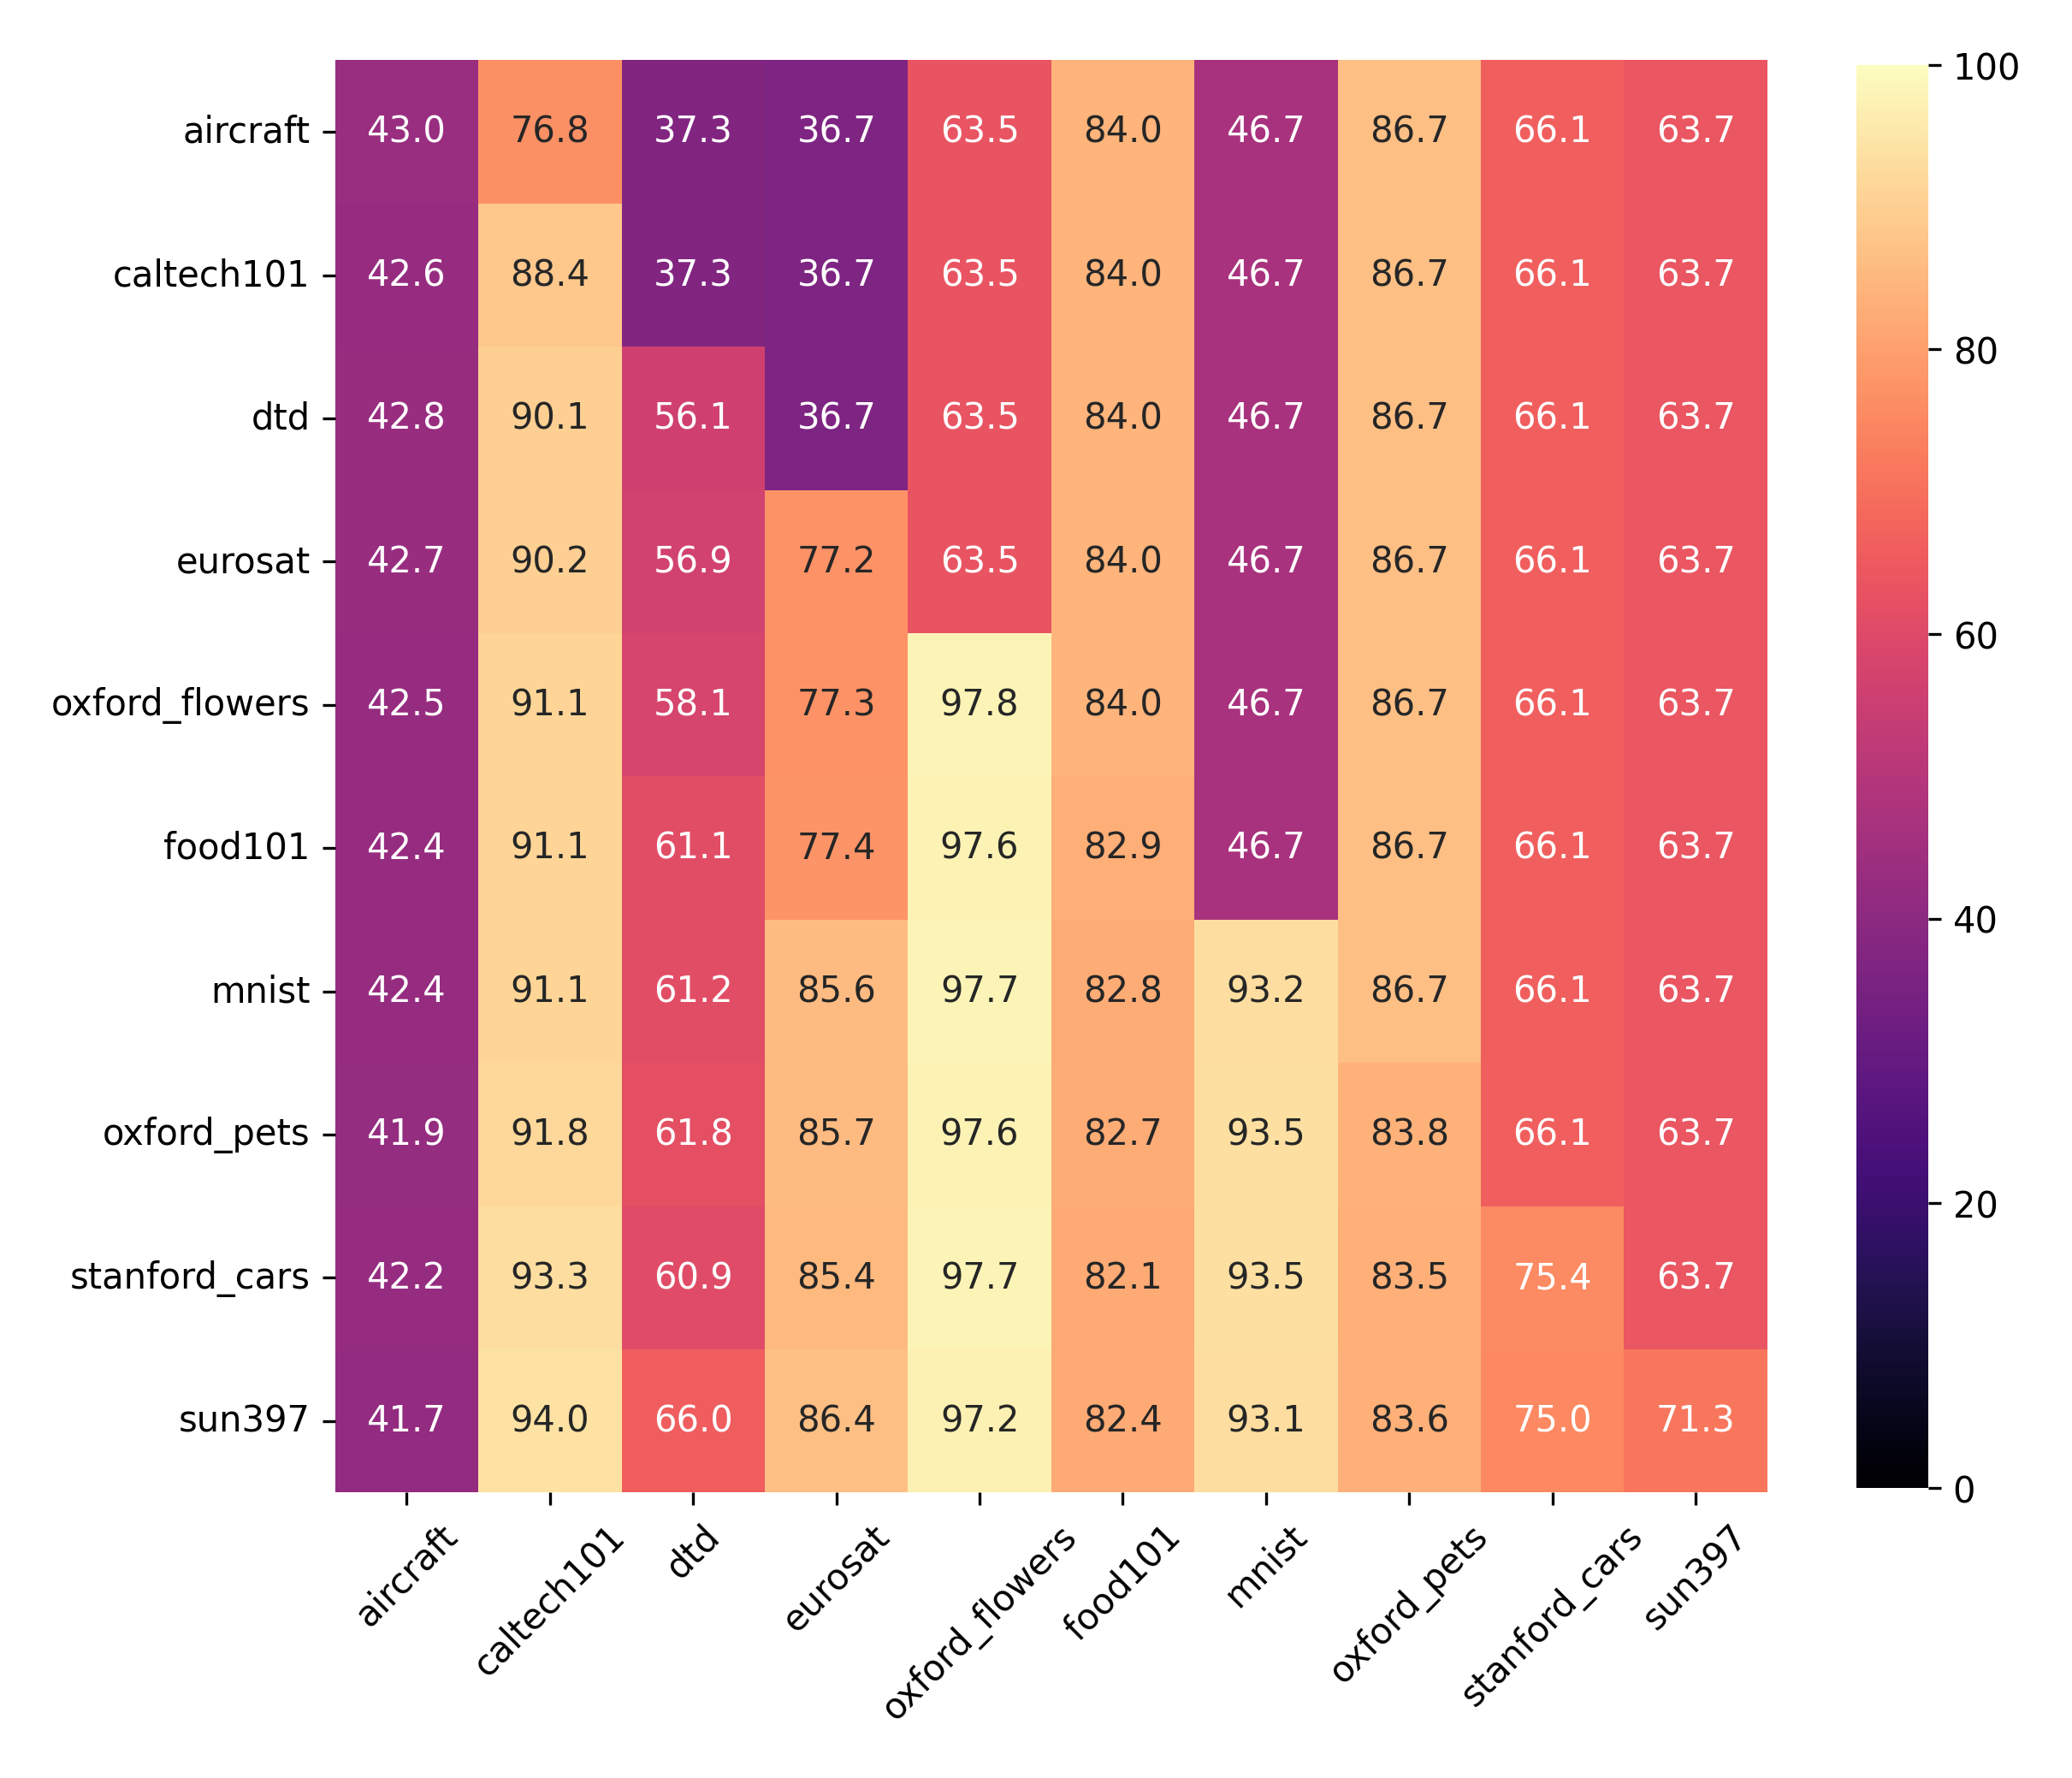
\includegraphics[width=\textwidth]{Figures/Primal_RAIL.png}
        \caption{Primal-RAIL}
    \end{subfigure}
    % \hfill
    \begin{subfigure}[b]{0.48\textwidth}
        \centering
        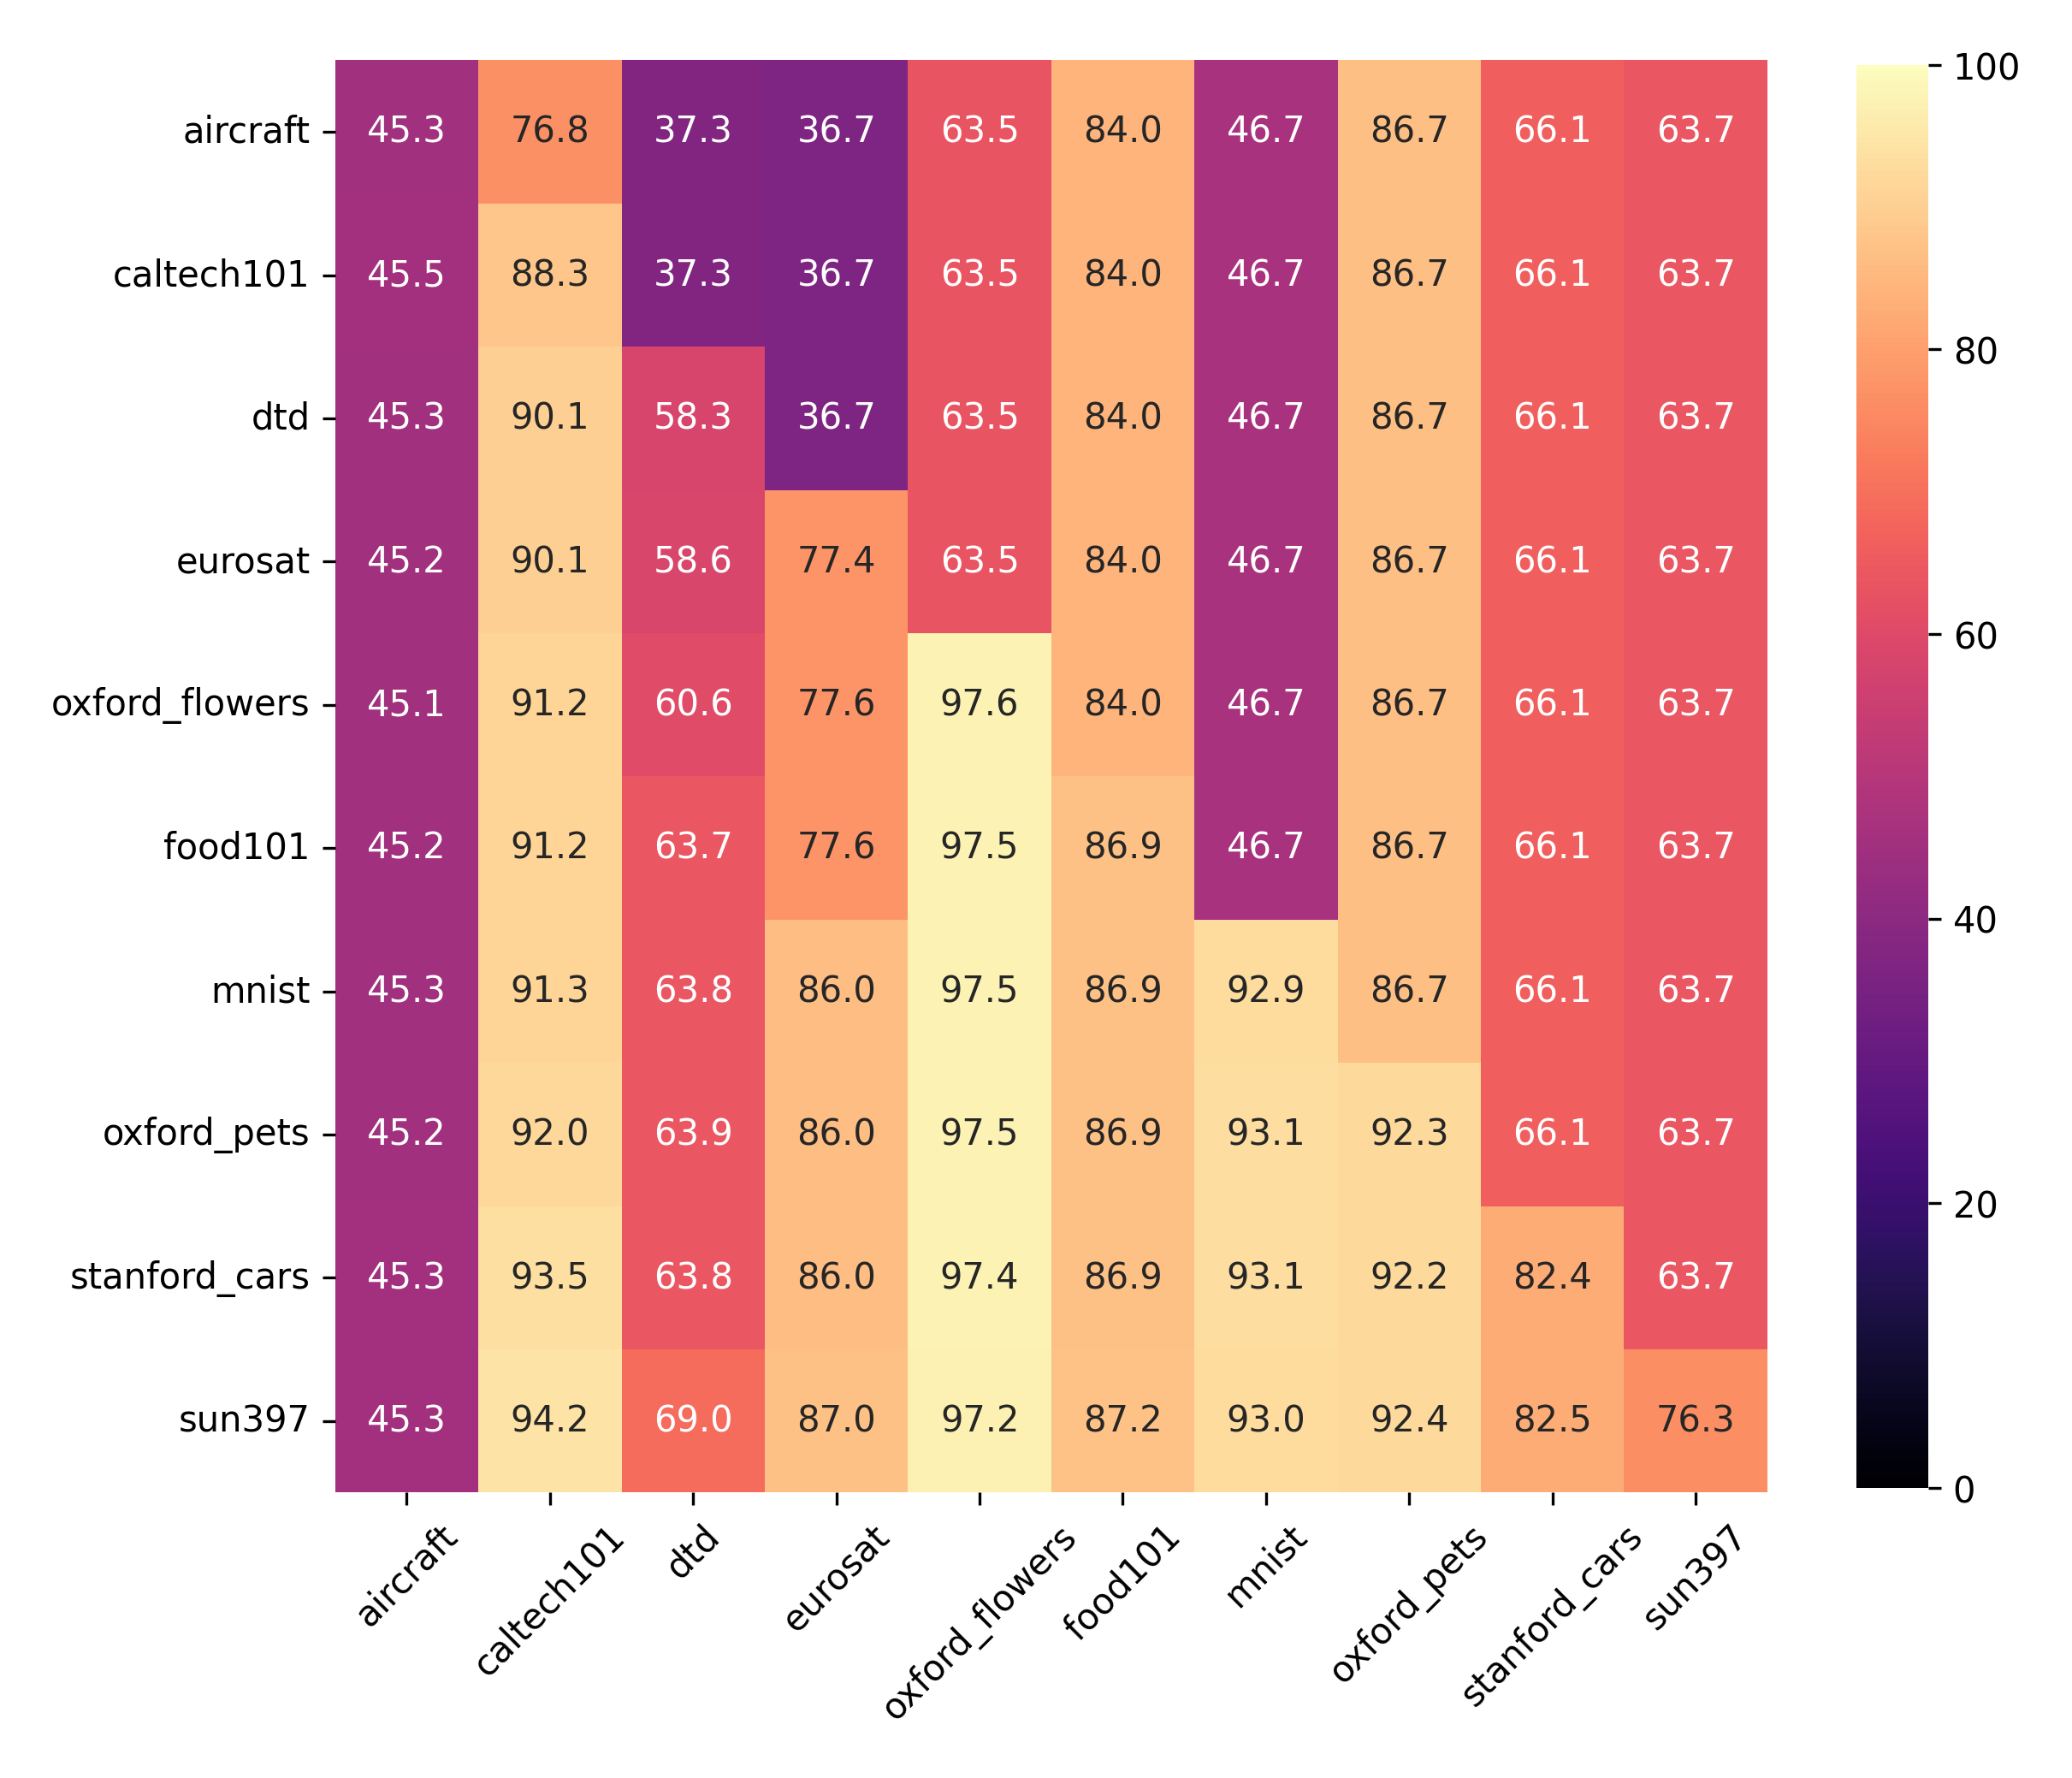
\includegraphics[width=\textwidth]{Figures/Dual_RAIL.png}
        \caption{Dual-RAIL}
    \end{subfigure}
    \caption{Accuracy (\%) of Primal-RAIL and Dual-RAIL in the X-TAIL setting with order-I. Each row denotes the performance on every domain after learning on one domain.}
    \label{fig:detailed_RAIL}
\end{figure}

In this section, we visualize the performance on each domain after every learning step in Fig.~\ref{fig:detailed_RAIL}. The upper-diagonal represents the performance before learning on the corresponding domain, which remains consistent with the zero-shot performance thanks to RAIL's absolute memorization of the zero-shot ability on unseen domains. On the other hand, the performance after learning a specific domain (lower-diagonal) does not degrades. Performance on some domains even improves with the learning step (e.g., Caltech-101), benefiting from our RAIL fusion module design, which reduces OOD errors as more domains are learned, thereby enhancing overall accuracy.

% \section{Comparison of different methods on full-shot MTIL setting}
% \label{app:mtil}
% In this section, we evaluate the performance of RAIL in full-shot MTIL setting, comparing it against the performance of baselines reported in~\cite{yu2024boosting}. In the context of MTIL, where the domain-identity is provided during testing, RAIL is reduced to the structure of multiple domain-specific classifiers trained on each domain separately. The domain-identity guides the test image to the corresponding classifier for within-domain prediction. As shown in~\ref{tab:full_mtil}, RAIL still surpasses all baseline methods in both primal and dual forms. This superior performance can be attributed to the non-linear projection, which significantly enhances the separability of features extracted by CLIP.

% \begin{table}
%     \centering
%     \footnotesize
%     \caption{Comparison with state-of-the-art methods on full-shot MTIL setting in terms of "Transfer", "Average", and "Last" scores (\%). The best results are highlighted with \textbf{bold} style.}
%     \label{tab:full_mtil}
%     \begin{tabular}{b{8em}b{1.6em}b{1.6em}b{1.6em}b{1.6em}b{1.6em}b{1.6em}b{1.6em}b{1.6em}b{1.6em}b{1.6em}b{1.6em}>{\centering\arraybackslash}m{3em}}
%     \toprule
%         \textbf{Method} &  \rot{Aircraft} &  \rot{Caltech101} & \rot{CIFAR100} &\rot{DTD} & \rot{EuroSAT} & \rot{Flower} & \rot{Food101} & \rot{MNIST} & \rot{Pets} & \rot{Cars} & \rot{Sun397} & \textbf{Average}\\
%     \midrule
%           \quad Zero-shot & 24.3 & 88.4 & 68.2 & 44.6 & 54.9 & 71.0 & 88.5 & 59.6 & 89.0 & 64.7 & 65.2 & {\cellcolor{lightgrey}}65.3\\
%           \quad Fine-tune & 62.0 & 95.1 & 89.6 & 79.5 & 98.9 & 97.5 & 92.7 & 99.6 & 94.7 & 89.6 & 81.8 & {\cellcolor{lightgrey}}89.2\\
%     \midrule
%         \multicolumn{11}{l}{\textbf{Transfer}}\\
%           \quad LwF & -- & 74.5 & 56.9 & 39.1 & 51.1 & 52.6 & 72.8 & 60.6 & 75.1 & 30.3 & 55.9 & {\cellcolor{lightgrey}} 58.9\\
%           \quad LwF-VR & -- & 77.1 & 61.0 & 40.5 & 45.3 & 54.4 & 74.6 & 47.9 & 76.7 & 36.3 & 58.6 & {\cellcolor{lightgrey}}57.2\\
%           \quad WiSE-FT & -- & 73.5 & 55.6 & 35.6 & 41.5 & 47.0 & 68.3 & 53.9 & 69.3 & 26.8 & 51.9 & {\cellcolor{lightgrey}}52.3\\
%           \quad ZSCL & -- & 86.0 & 67.4 & \textbf{45.4} & 50.4 & 69.1 & 87.6 & \textbf{61.8} & 86.8 & 60.1 & \textbf{66.8} & {\cellcolor{lightgrey}}68.1\\
%           \quad MoE-Adapter & -- & 87.9 & \textbf{68.2}& 44.4 & 49.9 & 70.7 & \textbf{88.7} & 59.7 & \textbf{89.1} & 64.5 & 65.5 & {\cellcolor{lightgrey}}68.9\\
%           \quad Primal-RAIL & -- & \textbf{88.4}&\textbf{68.2}& 44.6 &\textbf{54.9}&\textbf{71.0}& 88.5 & 59.6 & 89.0 &\textbf{64.7}&65.2& {\cellcolor{lightgrey}}\textbf{69.4}\\
%           % {\cellcolor{lightgrey}}\textbf{69.4(+0.5)}\\
%           \quad Dual-RAIL & -- & \textbf{88.4}&\textbf{68.2}& 44.6 &\textbf{54.9}&\textbf{71.0}& 88.5 & 59.6 & 89.0 &\textbf{64.7}&65.2& {\cellcolor{lightgrey}}\textbf{69.4}\\
%           % {\cellcolor{lightgrey}}\textbf{69.4(+0.5)}\\
          
%     \midrule
%         \multicolumn{11}{l}{\textbf{Average}}\\
%           \quad LwF& 36.3 & 86.9 & 72.0 & 59.0 & 73.7 & 60.0 & 73.6 & 74.8 & 80.0 & 37.3 & 58.1 & {\cellcolor{lightgrey}}64.7\\
%           \quad LwF-VR& 29.6 & 87.7 & 74.4 & 59.5 & 72.4 & 63.6 & 77.0 & 66.7 & 81.2 & 43.7 & 60.7 & {\cellcolor{lightgrey}}65.1\\
%           \quad WiSE-FT& 26.7 & 86.5 & 64.3 & 57.1 & 65.7 & 58.7 & 71.1 & 70.5 & 75.8 & 36.9 & 54.6 & {\cellcolor{lightgrey}}60.7\\
%           \quad ZSCL& 45.1 & 92.0 & 80.1 & 64.3 & 79.5 & 81.6 & \textbf{89.6} & \textbf{75.2} & 88.9 & 64.7 & \textbf{68.0} & {\cellcolor{lightgrey}}75.4\\
%           \quad MoE-Adapter & 50.2 & 91.9 & \textbf{83.1} & 69.4 & 78.9 & 84.0 & 89.1 & 73.7 & 89.3 & 67.7 & 66.9 & {\cellcolor{lightgrey}} 76.7\\
%           \quad Primal-RAIL & 51.9 & 95.8 & 80.1 & 70.3 & 81.1 & 86.1 & 89.0 & 73.9 & \textbf{90.2} & 68.4 & 66.4 & {\cellcolor{lightgrey}}77.6\\
%           % {\cellcolor{lightgrey}}71.9(+0.5)\\
%           \quad Dual-RAIL & \textbf{52.5} & \textbf{96.0} & 80.6 & \textbf{70.4} & \textbf{81.3} & \textbf{86.3} & 89.1 & 73.9 & \textbf{90.2} & \textbf{68.5} & 66.5 & {\cellcolor{lightgrey}}\textbf{77.8}
%           % {\cellcolor{lightgrey}}\textbf{72.3(+0.9)}
%  \\
%     \midrule
%         \multicolumn{11}{l}{\textbf{Last}}\\
%           \quad LwF& 26.3 & 87.5 & 71.9 & 66.6 & 79.9 & 66.9 & 83.8 & \textbf{99.6} & 92.1 & 66.1 & 80.4 & {\cellcolor{lightgrey}}74.6\\
%           \quad LwF-VR& 20.5 & 89.8 & 72.3 & 67.6 & 85.5 & 73.8 & 85.7 & \textbf{99.6} & 93.1 & 73.3 & 80.9 & {\cellcolor{lightgrey}}76.6\\
%           \quad WiSE-FT& 27.2 & 90.8 & 68.0 & 68.9 & 86.9 & 74.0 & 87.6 & \textbf{99.6} & 92.6 & 77.8 & \textbf{81.3} & {\cellcolor{lightgrey}}77.7\\
%           \quad ZSCL& 40.6 & 92.2 & 81.3 & 70.5 & 94.8 & 90.5 & \textbf{91.9} & 98.7 & \textbf{93.9} & 85.3 & 80.2 & {\cellcolor{lightgrey}}83.6\\
%           \quad MoE-Adapter & 49.8 & 92.2 & \textbf{86.1} & 78.1 & 95.7 & 94.3 & 89.5 & 98.1 & 89.9 & 81.6 & 80.0 & {\cellcolor{lightgrey}}85.0\\
%           \quad Primal-RAIL & 51.9 & 96.5 & 82.8 & 80.0 & 96.0 & 98.7 & 89.7 & 98.8 & 93.3 & 84.8 & 78.7 & {\cellcolor{lightgrey}}86.5\\
%           % {\cellcolor{lightgrey}}77.2(+1.1)\\
%           \quad Dual-RAIL & \textbf{52.5} & \textbf{96.8} & 83.3 & \textbf{80.1} & \textbf{96.4} & \textbf{99.0} & 89.9 & 98.8 & 93.5 & \textbf{85.5} & 79.2 & {\cellcolor{lightgrey}}\textbf{86.8} \\
%           % {\cellcolor{lightgrey}}\textbf{77.9(+1.8)} \\
%     \bottomrule
%     \end{tabular}
% \end{table}

% \begin{table}[h]
%     \centering
%     \caption{Accuracy(\%) of the LwF method on X-TAIL with order-I.}
%     \label{tab:lwf_fs_merged}
%     \begin{tabular}{b{5em}b{2em}b{2em}b{2em}b{2em}b{2em}b{2em}b{2em}b{2em}b{2em}b{2em}b{2em}}
%     \toprule
%         &  \rot{Aircraft} &  \rot{Caltech101} & \rot{DTD} & \rot{EuroSAT} & \rot{Flower} & \rot{Food101} & \rot{MNIST} & \rot{Pets} & \rot{Cars} & \rot{Sun397} & \\
%         \midrule
% \textbf{Transfer} & nan & 66.6 & 26.9 & 19.5 & 51.0 & 78.4 & 26.6 & 68.9 & 35.5 & 56.1 & \cellcolor{blue!25}\textbf{47.7}\\
% \midrule
% Aircraft & 35.1 & 66.6 & 26.6 & 23.8 & 47.5 & 78.0 & 25.7 & 70.8 & 32.6 & 59.2\\
% Caltech101 & 26.1 & 85.3 & 27.1 & 21.3 & 55.0 & 80.4 & 27.2 & 72.0 & 38.6 & 62.1\\
% DTD & 25.1 & 83.9 & 49.3 & 13.3 & 53.6 & 79.2 & 28.2 & 76.9 & 39.3 & 57.6\\
% EuroSAT & 29.3 & 77.8 & 46.6 & 44.9 & 48.0 & 78.0 & 30.4 & 77.3 & 37.7 & 50.7\\
% Flowers & 27.4 & 79.6 & 45.4 & 50.3 & 91.9 & 76.5 & 22.6 & 71.5 & 33.2 & 52.8\\
% Food & 20.3 & 84.6 & 34.3 & 51.7 & 58.3 & 83.8 & 25.4 & 52.4 & 33.1 & 55.9\\
% MNIST & 17.6 & 84.3 & 39.7 & 47.2 & 69.7 & 82.7 & 40.9 & 61.4 & 35.5 & 56.7\\
% OxfordPet & 20.2 & 80.5 & 35.1 & 32.4 & 73.5 & 81.5 & 31.5 & 73.0 & 34.2 & 53.3\\
% StanfordCars & 20.6 & 82.2 & 39.6 & 29.2 & 76.1 & 82.3 & 51.1 & 75.4 & 78.7 & 56.9\\
% SUN397 & 20.9 & 83.1 & 47.5 & 38.2 & 75.5 & 84.7 & 50.1 & 78.0 & 75.8 & 74.6 & \cellcolor{orange!25}\textbf{62.8}\\
% \midrule
% \textbf{Average} & 24.3 & 80.8 & 39.1 & 35.2 & 64.9 & 80.7 & 33.3 & 70.9 & 43.9 & 58.0 & \cellcolor{red!25}\textbf{53.1}\\
%     \bottomrule
%     \end{tabular}
% \end{table}

% \begin{table}[h]
%     \centering
%     \caption{Accuracy(\%) of the WiSE-FT method on X-TAIL with order-I.}
%     \label{tab:lwf_fs_merged}
%     \begin{tabular}{b{5em}b{2em}b{2em}b{2em}b{2em}b{2em}b{2em}b{2em}b{2em}b{2em}b{2em}b{2em}}
%     \toprule
%         &  \rot{Aircraft} &  \rot{Caltech101} & \rot{DTD} & \rot{EuroSAT} & \rot{Flower} & \rot{Food101} & \rot{MNIST} & \rot{Pets} & \rot{Cars} & \rot{Sun397} & \\
%         \midrule
% \textbf{Transfer} & -- & 70.1 & 31.9 & 25.3 & 56.3 & 79.8 & 29.9 & 74.9 & 45.6 & 56.8 & \cellcolor{blue!25}\textbf{52.3}\\
% \midrule
% Aircraft & 31.9 & 70.1 & 33.2 & 31.9 & 60.1 & 84.1 & 30.9 & 82.6 & 51.1 & 63.5\\
% Caltech101 & 30.2 & 81.3 & 30.5 & 24.1 & 56.8 & 81.4 & 29.0 & 76.8 & 50.1 & 61.2\\
% DTD & 28.7 & 79.2 & 50.1 & 20.0 & 54.3 & 78.2 & 29.7 & 77.1 & 48.4 & 55.8\\
% EuroSAT & 30.8 & 77.6 & 48.6 & 38.7 & 53.9 & 79.3 & 31.6 & 77.2 & 47.8 & 52.8\\
% Flowers & 26.7 & 77.9 & 43.3 & 46.3 & 88.4 & 76.1 & 29.5 & 70.1 & 40.3 & 52.3\\
% Food & 27.4 & 77.5 & 41.9 & 41.0 & 72.5 & 84.0 & 28.9 & 67.7 & 44.3 & 59.5\\
% MNIST & 26.7 & 76.4 & 42.7 & 37.6 & 74.3 & 83.5 & 40.2 & 73.2 & 43.9 & 57.8\\
% OxfordPet & 24.3 & 74.0 & 37.3 & 29.3 & 74.8 & 81.9 & 32.9 & 72.6 & 38.9 & 53.1\\
% StanfordCars & 23.1 & 74.4 & 38.6 & 23.4 & 74.1 & 82.3 & 30.2 & 72.8 & 76.2 & 55.4\\
% SUN397 & 21.8 & 76.8 & 42.9 & 20.8 & 77.5 & 84.9 & 30.7 & 76.6 & 75.8 & 72.5 & \cellcolor{orange!25}\textbf{58.0}\\
% \midrule
% \textbf{Average} & 27.1 & 76.5 & 40.9 & 31.3 & 68.7 & 81.6 & 31.4 & 74.7 & 51.7 & 58.4 & \cellcolor{red!25}\textbf{54.2}\\
%     \bottomrule
%     \end{tabular}
% \end{table}

% \begin{table}[h]
%     \centering
%     \caption{Accuracy(\%) of the iCaRL method on X-TAIL with order-I.}
%     \label{tab:lwf_fs_merged}
%     \begin{tabular}{b{5em}b{2em}b{2em}b{2em}b{2em}b{2em}b{2em}b{2em}b{2em}b{2em}b{2em}b{2em}}
%     \toprule
%         &  \rot{Aircraft} &  \rot{Caltech101} & \rot{DTD} & \rot{EuroSAT} & \rot{Flower} & \rot{Food101} & \rot{MNIST} & \rot{Pets} & \rot{Cars} & \rot{Sun397} & \\
%         \midrule
% \textbf{Transfer} & nan & 71.7 & 35.0 & 43.0 & 64.4 & 86.9 & 43.9 & 87.8 & 63.7 & 60.0 & \cellcolor{blue!25}\textbf{61.8}\\
% \midrule
% Aircraft & 25.3 & 71.7 & 34.7 & 43.5 & 63.6 & 86.7 & 42.7 & 87.1 & 63.7 & 58.6\\
% Caltech101 & 25.4 & 72.1 & 35.3 & 42.6 & 64.4 & 86.9 & 43.4 & 87.6 & 63.8 & 59.4\\
% DTD & 25.4 & 72.2 & 37.6 & 42.8 & 64.8 & 87.0 & 43.5 & 87.9 & 63.8 & 59.8\\
% EuroSAT & 25.5 & 72.3 & 37.8 & 55.2 & 64.8 & 87.0 & 44.6 & 87.9 & 63.7 & 60.1\\
% Flowers & 25.4 & 72.1 & 37.7 & 55.2 & 65.7 & 87.0 & 44.4 & 88.0 & 63.7 & 60.0\\
% Food & 25.4 & 72.0 & 37.6 & 55.1 & 65.8 & 87.0 & 44.5 & 88.0 & 63.7 & 60.1\\
% MNIST & 25.6 & 72.4 & 38.2 & 55.4 & 65.5 & 87.2 & 81.9 & 88.1 & 63.6 & 60.8\\
% OxfordPet & 25.5 & 72.2 & 38.5 & 55.5 & 65.5 & 87.2 & 81.9 & 88.7 & 63.6 & 60.5\\
% StanfordCars & 25.2 & 71.9 & 38.7 & 55.3 & 65.5 & 87.3 & 81.8 & 88.6 & 63.6 & 60.3\\
% SUN397 & 25.5 & 72.1 & 38.9 & 55.4 & 65.5 & 87.3 & 81.9 & 88.6 & 63.6 & 61.5 & \cellcolor{orange!25}\textbf{64.0}\\
% \midrule
% \textbf{Average} & 25.4 & 72.1 & 37.5 & 51.6 & 65.1 & 87.1 & 59.1 & 88.0 & 63.7 & 60.1 & \cellcolor{red!25}\textbf{61.0}\\
%     \bottomrule
%     \end{tabular}
% \end{table}

% \begin{table}[h]
%     \centering
%     \caption{Accuracy(\%) of the ZSCL method on X-TAIL with order-I.}
%     \label{tab:lwf_fs_merged}
%     \begin{tabular}{b{5em}b{2em}b{2em}b{2em}b{2em}b{2em}b{2em}b{2em}b{2em}b{2em}b{2em}b{2em}}
%     \toprule
%         &  \rot{Aircraft} &  \rot{Caltech101} & \rot{DTD} & \rot{EuroSAT} & \rot{Flower} & \rot{Food101} & \rot{MNIST} & \rot{Pets} & \rot{Cars} & \rot{Sun397} & \\
%         \midrule
% \textbf{Transfer} & -- & 73.3 & 32.6 & 36.8 & 62.1 & 83.8 & 42.1 & 83.6 & 56.5 & 60.2 & \cellcolor{blue!25}\textbf{59.0}\\
% \midrule
% Aircraft & 42.7 & 73.3 & 34.9 & 42.3 & 65.5 & 86.7 & 43.9 & 86.5 & 61.7 & 62.7\\
% Caltech101 & 40.7 & 77.0 & 30.2 & 34.7 & 62.5 & 84.3 & 38.9 & 82.0 & 58.8 & 61.6\\
% DTD & 40.2 & 75.5 & 48.1 & 33.3 & 60.4 & 83.0 & 41.1 & 83.9 & 57.8 & 60.3\\
% EuroSAT & 39.3 & 73.2 & 48.4 & 50.6 & 59.8 & 82.7 & 42.2 & 84.0 & 56.9 & 58.1\\
% Flowers & 36.2 & 73.5 & 42.2 & 43.7 & 85.6 & 82.3 & 41.5 & 80.0 & 52.7 & 56.2\\
% Food & 34.3 & 77.1 & 42.7 & 47.6 & 77.1 & 87.4 & 44.7 & 84.2 & 56.1 & 62.7\\
% MNIST & 34.4 & 76.1 & 43.5 & 45.3 & 77.8 & 87.3 & 56.8 & 84.7 & 55.8 & 61.9\\
% OxfordPet & 29.7 & 74.9 & 37.4 & 36.0 & 74.7 & 86.0 & 51.9 & 82.2 & 52.3 & 58.7\\
% StanfordCars & 29.9 & 74.0 & 36.4 & 36.2 & 72.0 & 86.1 & 51.7 & 81.4 & 77.9 & 59.4\\
% SUN397 & 33.1 & 75.3 & 43.5 & 35.2 & 74.6 & 87.4 & 50.4 & 84.2 & 77.3 & 73.4 & \cellcolor{orange!25}\textbf{63.4}\\
% \midrule
% \textbf{Average} & 36.0 & 75.0 & 40.7 & 40.5 & 71.0 & 85.3 & 46.3 & 83.3 & 60.7 & 61.5 & \cellcolor{red!25}\textbf{60.0}\\
%     \bottomrule
%     \end{tabular}
% \end{table}

% \begin{table}[h]
%     \centering
%     \caption{Accuracy(\%) of the MoE-Adapter method on X-TAIL with order-I.}
%     \label{tab:lwf_fs_merged}
%     \begin{tabular}{b{5em}b{2em}b{2em}b{2em}b{2em}b{2em}b{2em}b{2em}b{2em}b{2em}b{2em}b{2em}}
%     \toprule
%         &  \rot{Aircraft} &  \rot{Caltech101} & \rot{DTD} & \rot{EuroSAT} & \rot{Flower} & \rot{Food101} & \rot{MNIST} & \rot{Pets} & \rot{Cars} & \rot{Sun397} & \\
%         \midrule
% \textbf{Transfer} & -- & 71.0 & 34.9 & 19.2 & 63.0 & 86.6 & 20.0 & 87.2 & 63.7 & 58.6 & \cellcolor{blue!25}\textbf{56.0}\\
% \midrule
% Aircraft & 43.3 & 71.0 & 35.5 & 19.2 & 64.0 & 86.6 & 12.6 & 87.2 & 63.7 & 58.3\\
% Caltech101 & 43.7 & 79.7 & 34.3 & 19.2 & 62.5 & 86.6 & 16.0 & 87.2 & 63.7 & 58.6\\
% DTD & 43.5 & 78.7 & 58.6 & 19.2 & 62.7 & 86.6 & 22.7 & 87.2 & 63.7 & 58.8\\
% EuroSAT & 43.3 & 78.3 & 56.4 & 48.5 & 62.9 & 86.6 & 22.1 & 87.2 & 63.7 & 58.8\\
% Flowers & 43.8 & 78.3 & 58.2 & 47.1 & 92.2 & 86.6 & 23.1 & 87.2 & 63.7 & 58.6\\
% Food & 43.7 & 78.4 & 55.4 & 41.9 & 88.9 & 86.2 & 23.3 & 87.2 & 63.7 & 58.6\\
% MNIST & 44.0 & 78.5 & 54.0 & 43.1 & 87.6 & 86.1 & 82.1 & 87.2 & 63.7 & 58.6\\
% OxfordPet & 43.7 & 78.4 & 54.8 & 40.1 & 80.7 & 85.8 & 82.0 & 87.9 & 63.7 & 58.5\\
% StanfordCars & 43.2 & 78.6 & 55.8 & 36.0 & 78.3 & 86.0 & 81.7 & 87.9 & 78.1 & 58.5\\
% SUN397 & 43.2 & 78.7 & 57.6 & 32.8 & 79.4 & 86.0 & 86.7 & 87.8 & 78.2 & 74.2 & \cellcolor{orange!25}\textbf{70.5}\\
% \midrule
% \textbf{Average} & 43.6 & 77.9 & 52.1 & 34.7 & 75.9 & 86.3 & 45.2 & 87.4 & 66.6 & 60.2 & \cellcolor{red!25}\textbf{63.0}\\
%     \bottomrule
%     \end{tabular}
% \end{table}

% \clearpage
% \begin{table}
%     \centering
%     \caption{Comparison of different CL methods on X-TAIL setting with order II.}
%     \label{tab:main_table_order2}
%     \begin{tabular}{b{6em}b{3em}b{3em}b{3em}}
%     \toprule
%         Method & Transfer & Average & Last\\
%     \midrule
%         LwF & 46.9 & 52.0 & 55.4\\
%         WiSE-FT & 51.1 & 56.9 & 61.5\\
%         iCaRL &  &  & \\
%         ZSCL & 56.9 & 63.6 & 69.4\\ 
%         MoE-Adapter & & & \\
%         Ours (Primal) & & & \\
%         Ours (Dual) & & & \\
%     \bottomrule
%     \end{tabular}
% \end{table}

\section{Comparison of different methods on X-TAIL with order II.}
\label{app:order2}
In this section, we compare different methods in X-TAIL setting with a random order: StanfordCars, Aircraft, OxfordPet, Food, SUN397, MNIST, Flowers, DTD, Caltech101, EuroSAT. As shown in Tab.~\ref{tab:detailed_comparison_order2}, our method again outperforms previous methods on all metrics, reinforcing the conclusions presented in Sec.~\ref{sec:comparison}.

\begin{table}
    \centering
    \footnotesize
    \caption{Comparison of different CL methods on X-TAIL for each domain with order II in terms of "Transfer", "Average", and "Last" scores (\%). The best results are highlighted with \textbf{bold} style.}
    \label{tab:detailed_comparison_order2}
    \begin{tabular}{b{8em}b{1.6em}b{1.6em}b{1.6em}b{1.6em}b{1.6em}b{1.6em}b{1.6em}b{1.6em}b{1.6em}b{1.6em}>{\centering\arraybackslash}m{3em}}
    \toprule
        \textbf{Method} &  \rot{Cars} &  \rot{Aircraft} & \rot{Pets} & \rot{Food} & \rot{SUN397} & \rot{MNIST} & \rot{Flower} & \rot{DTD} & \rot{Caltech101} & \rot{EuroSAT} & \textbf{Average} \\
    \midrule
          \quad Zero-shot & 66.1 & 23.5 & 86.7 & 84.0 & 63.7 & 46.7 & 63.6 & 37.3 & 76.8 & 36.7 & {\cellcolor{lightgrey}}58.5 \\
          \quad Fine-tune & 77.4 & 39.6 & 84.4 & 85.5 & 72.4 & 95.1 & 95.4 & 68.2 & 93.3 & 89.2 & {\cellcolor{lightgrey}}80.1 \\
    \midrule
        \multicolumn{11}{l}{\textbf{Transfer}}\\
          \quad LwF& -- & 20.0 & 74.1 & 79.6 & 58.1 & 34.1 & 48.9 & 27.7 & 64.4 & 15.1 & {\cellcolor{lightgrey}}46.9\\
          \quad WiSE-FT & -- & 21.3 & 79.5 & 83.3 & 61.0 & 39.9 & 56.5 & 29.6 & 68.0 & 20.8 & {\cellcolor{lightgrey}}51.1\\
          % \quad iCaRL& -- &  &  &  &  &  &  &  & & \\
          \quad ZSCL & -- & 23.0 & 84.3 & 87.2 & 63.0 & 42.1 & 65.2 & 34.6 & 71.4 & \textbf{40.9} & {\cellcolor{lightgrey}}56.9\\
          \quad MoE-Adapter & -- & 17.1 & \textbf{87.2} & \textbf{87.5} & 58.4 & 12.6 & \textbf{65.5} & 35.9 & 70.0 & 17.9& {\cellcolor{lightgrey}}50.2\\
          \quad Primal-RAIL & -- & \textbf{23.5} & 86.7 & 84.0 & \textbf{63.7} & \textbf{46.7} & 63.5 & \textbf{37.3} & \textbf{76.8} & 36.7 & {\cellcolor{lightgrey}}\textbf{57.7}\\
          \quad Dual-RAIL & -- & \textbf{23.5} & 86.7 & 84.0 & \textbf{63.7} & \textbf{46.7} & 63.5 & \textbf{37.3} & \textbf{76.8} & 36.7 & {\cellcolor{lightgrey}}\textbf{57.7}\\
    \midrule
        \multicolumn{11}{l}{\textbf{Average}}\\
          \quad LwF& 49.0 & 27.4 & 69.7 & 83.0 & 65.7 & 42.2 & 63.5 & 33.1 & 68.5 & 17.5 & {\cellcolor{lightgrey}}52.0\\
          \quad WiSE-FT & 57.9 & 29.6 & 77.8 & 85.4 & 68.0 & 51.6 & 69.3 & 35.5 & 71.0 & 23.0 & {\cellcolor{lightgrey}}56.9\\
          % \quad iCaRL& -- &  &  &  &  &  &  &  & & \\
          \quad ZSCL & 74.4 & 36.4 & 86.7 & \textbf{88.7} & 68.9 & 50.0 & 75.1 & 40.1 & 72.5 & \textbf{43.7} & {\cellcolor{lightgrey}}63.6\\
          \quad MoE-Adapter & 74.4 & 38.6 & 87.7 & 87.3 & 67.9 & 50.6 & 76.5 & 43.7 & 72.3 & 18.8& {\cellcolor{lightgrey}}61.8\\
          \quad Primal-RAIL & 77.9 & 40.4 & 85.6 & 83.3 & 68.3 & 62.2 & 76.6 & 45.8 & \textbf{80.4} & 41.7 & {\cellcolor{lightgrey}}66.2\\
          \quad Dual-RAIL & \textbf{82.3} & \textbf{43.4} & \textbf{90.4} & 86.0 & \textbf{71.0} & \textbf{62.8} & \textbf{76.7} & \textbf{46.7} & 80.3& 41.7 & {\cellcolor{lightgrey}}\textbf{68.1}\\
    \midrule
        \multicolumn{11}{l}{\textbf{Last}}\\ 
          \quad LwF& 29.6 & 17.5 & 63.0 & 83.8 & 67.7 & 44.9 & 79.3 & 44.8 & 84.6 & 39.0 & {\cellcolor{lightgrey}}55.4\\ 
          \quad WiSE-FT & 46.1 & 23.5 & 71.3 & 85.7 & 70.2 & 59.1 & 85.5 & 47.9 & 82.4 & 42.8 & {\cellcolor{lightgrey}}61.5\\ 
          % \quad iCaRL& -- &  &  &  &  &  &  &  &  & \\ 
          \quad ZSCL & 71.7 & 35.3 & 86.5 & \textbf{89.2} & 71.8 & 52.3 & 89.8 & 52.0 & 77.1 & 68.4 & {\cellcolor{lightgrey}}69.4\\ 
          \quad MoE-Adapter & 75.1 & 41.1 & 87.9 & 87.1 & 74.1 & 89.7 & 92.6 & 61.2 & 81.0 & 27.4& {\cellcolor{lightgrey}}71.7\\ 
          \quad Primal-RAIL & 77.7 & 41.9 & 86.1 & 83.3 & 71.8 & 91.6 & 97.3 & 66.4 & \textbf{94.8} & 86.9 & {\cellcolor{lightgrey}}79.8\\ 
          \quad Dual-RAIL & \textbf{82.3} & \textbf{45.8} & \textbf{92.0} & 87.1 & \textbf{76.3} & \textbf{93.1} & \textbf{97.4} & \textbf{69.1} & 94.4 & \textbf{87.1} & {\cellcolor{lightgrey}}\textbf{82.5}\\
    \bottomrule
    \end{tabular}
\end{table}

% \begin{table}[h]
%     \centering
%     \caption{Accuracy(\%) of the LwF method on X-TAIL with order-II.}
%     \label{tab:xtail_order_2}
%     \begin{tabular}{b{5em}b{2em}b{2em}b{2em}b{2em}b{2em}b{2em}b{2em}b{2em}b{2em}b{2em}b{2em}}
%     \toprule
%         &  \rot{StanfordCars} &  \rot{Aircraft} & \rot{OxfordPet} & \rot{Food} & \rot{SUN397} & \rot{MNIST} & \rot{Flowers} & \rot{DTD} & \rot{Caltech101} & \rot{EuroSAT} & \\
%         \midrule
% \textbf{Transfer} & -- & 20.0 & 74.1 & 79.6 & 58.1 & 34.1 & 48.9 & 27.7 & 64.4 & 15.1 & \cellcolor{blue!25}\textbf{46.9}\\
% \midrule
% StanfordCars & 79.7 & 20.0 & 84.6 & 87.3 & 63.0 & 38.2 & 61.7 & 34.9 & 69.6 & 39.5\\
% Aircraft & 40.5 & 35.8 & 63.5 & 73.6 & 57.3 & 27.7 & 41.8 & 23.1 & 62.1 & 11.3\\
% OxfordPet & 50.0 & 34.5 & 73.8 & 78.0 & 57.5 & 29.2 & 49.2 & 25.0 & 61.4 & 19.1\\
% Food & 42.5 & 31.9 & 54.5 & 84.5 & 54.4 & 37.6 & 37.9 & 17.9 & 62.4 & 19.9\\
% SUN397 & 62.4 & 31.5 & 76.1 & 86.0 & 74.8 & 37.9 & 51.7 & 32.0 & 69.5 & 17.5\\
% MNIST & 58.4 & 30.6 & 75.9 & 85.4 & 73.5 & 69.4 & 50.9 & 30.2 & 66.3 & 16.6\\
% Flowers & 51.1 & 30.7 & 72.5 & 84.5 & 71.4 & 60.2 & 93.3 & 31.0 & 63.8 & 7.5\\
% DTD & 44.9 & 28.6 & 65.6 & 83.3 & 66.9 & 41.8 & 88.9 & 46.1 & 60.3 & 3.5\\
% Caltech101 & 31.1 & 12.7 & 67.6 & 83.8 & 70.5 & 34.7 & 79.7 & 45.8 & 85.1 & 1.0\\
% EuroSAT & 29.6 & 17.5 & 63.0 & 83.8 & 67.7 & 44.9 & 79.3 & 44.8 & 84.6 & 39.0 & \cellcolor{orange!25}\textbf{55.4}\\
% \midrule
% \textbf{Average} & 49.0 & 27.4 & 69.7 & 83.0 & 65.7 & 42.2 & 63.5 & 33.1 & 68.5 & 17.5 & \cellcolor{red!25}\textbf{52.0}\\
%     \bottomrule
%     \end{tabular}
% \end{table}

% \begin{table}[h]
%     \centering
%     \caption{Accuracy(\%) of the WiSE-FT method on X-TAIL with order-II.}
%     \label{tab:xtail_order_2}
%     \begin{tabular}{b{5em}b{2em}b{2em}b{2em}b{2em}b{2em}b{2em}b{2em}b{2em}b{2em}b{2em}b{2em}}
%     \toprule
%         &  \rot{StanfordCars} &  \rot{Aircraft} & \rot{OxfordPet} & \rot{Food} & \rot{SUN397} & \rot{MNIST} & \rot{Flowers} & \rot{DTD} & \rot{Caltech101} & \rot{EuroSAT} & \\
%         \midrule
% \textbf{Transfer} & -- & 21.3 & 79.5 & 83.3 & 61.0 & 39.9 & 56.5 & 29.6 & 68.0 & 20.8 & \cellcolor{blue!25}\textbf{51.1}\\
% \midrule
% StanfordCars & 80.6 & 21.3 & 84.4 & 87.5 & 61.8 & 37.1 & 63.1 & 35.1 & 70.2 & 43.2\\
% Aircraft & 51.9 & 36.8 & 74.6 & 80.4 & 60.0 & 35.5 & 55.9 & 27.8 & 67.8 & 11.0\\
% OxfordPet & 57.1 & 36.6 & 82.9 & 82.0 & 61.8 & 38.0 & 56.8 & 28.2 & 67.8 & 16.6\\
% Food & 50.7 & 33.8 & 65.5 & 86.4 & 60.6 & 43.5 & 46.0 & 21.7 & 65.3 & 24.5\\
% SUN397 & 63.6 & 32.5 & 80.5 & 87.1 & 74.8 & 45.5 & 58.1 & 30.5 & 70.2 & 27.7\\
% MNIST & 63.7 & 30.4 & 82.0 & 86.8 & 73.8 & 75.7 & 59.0 & 32.2 & 69.0 & 25.5\\
% Flowers & 59.5 & 31.6 & 81.8 & 86.4 & 73.2 & 69.4 & 91.6 & 31.3 & 67.6 & 18.8\\
% DTD & 56.3 & 30.5 & 79.8 & 85.9 & 71.2 & 59.6 & 90.9 & 52.3 & 66.0 & 11.1\\
% Caltech101 & 49.5 & 19.4 & 74.7 & 85.7 & 72.4 & 52.4 & 86.1 & 47.7 & 83.4 & 8.9\\
% EuroSAT & 46.1 & 23.5 & 71.3 & 85.7 & 70.2 & 59.1 & 85.5 & 47.9 & 82.4 & 42.8 & \cellcolor{orange!25}\textbf{61.5}\\
% \midrule
% \textbf{Average} & 57.9 & 29.6 & 77.8 & 85.4 & 68.0 & 51.6 & 69.3 & 35.5 & 71.0 & 23.0 & \cellcolor{red!25}\textbf{56.9}\\
%     \bottomrule
%     \end{tabular}
% \end{table}

% \begin{table}[h]
%     \centering
%     \caption{Accuracy(\%) of the ZSCL method on X-TAIL with order-II.}
%     \label{tab:lwf_fs_merged_order2}
%     \begin{tabular}{b{5em}b{2em}b{2em}b{2em}b{2em}b{2em}b{2em}b{2em}b{2em}b{2em}b{2em}b{2em}}
%     \toprule
%         &  \rot{StanfordCars} &  \rot{Aircraft} & \rot{OxfordPet} & \rot{Food} & \rot{SUN397} & \rot{MNIST} & \rot{Flowers} & \rot{DTD} & \rot{Caltech101} & \rot{EuroSAT} & \\
%         \midrule
% \textbf{Transfer} & -- & 23.0 & 84.3 & 87.2 & 63.0 & 42.1 & 65.2 & 34.6 & 71.4 & 40.9 & \cellcolor{blue!25}\textbf{56.9}\\
% \midrule
% StanfordCars & 79.9 & 23.0 & 85.6 & 87.7 & 60.6 & 37.5 & 63.7 & 35.4 & 70.1 & 44.8\\
% Aircraft & 72.1 & 40.3 & 83.0 & 86.9 & 63.4 & 41.1 & 64.0 & 34.6 & 71.3 & 39.8\\
% OxfordPet & 75.7 & 40.2 & 89.6 & 87.0 & 64.1 & 40.0 & 66.6 & 34.0 & 72.5 & 37.2\\
% Food & 74.1 & 38.9 & 84.1 & 89.3 & 63.8 & 44.3 & 63.1 & 29.9 & 71.3 & 39.3\\
% SUN397 & 75.3 & 38.9 & 87.8 & 89.6 & 73.7 & 47.5 & 66.5 & 34.1 & 72.2 & 41.4\\
% MNIST & 75.5 & 38.3 & 87.8 & 89.4 & 73.1 & 66.3 & 67.1 & 36.5 & 72.2 & 40.9\\
% Flowers & 74.3 & 38.3 & 87.8 & 89.2 & 73.2 & 64.8 & 90.3 & 37.8 & 71.6 & 40.5\\
% DTD & 73.1 & 37.4 & 88.3 & 89.4 & 71.9 & 51.7 & 90.6 & 56.5 & 69.8 & 42.5\\
% Caltech101 & 72.6 & 33.6 & 86.2 & 89.2 & 72.9 & 54.1 & 89.0 & 50.5 & 76.8 & 41.7\\
% EuroSAT & 71.7 & 35.3 & 86.5 & 89.2 & 71.8 & 52.3 & 89.8 & 52.0 & 77.1 & 68.4 & \cellcolor{orange!25}\textbf{69.4}\\
% \midrule
% \textbf{Average} & 74.4 & 36.4 & 86.7 & 88.7 & 68.9 & 50.0 & 75.1 & 40.1 & 72.5 & 43.7 & \cellcolor{red!25}\textbf{63.6}\\
%     \bottomrule
%     \end{tabular}
% \end{table}

% \begin{table}[h!]
% \centering
% \caption{Real time execution of models}
% \renewcommand{\arraystretch}{1.5} % Adjust line spacing
% \begin{tabular}{lc}
% \hline
% \textbf{Model} & \textbf{Real time} \\
% \hline
% ZSCL & 514m 40.163s \\
% Moe-Adapter & 47m 2.319s \\
% Primal-RAIL & 4m 0.071s \\
% Dual-RAIL & 4m 13.200s \\
% \hline
% \end{tabular}
% \label{tab:real_time}
% \end{table}



\section{Limitation}
\label{app:limitation}
RAIL exhibits its superior performance and efficiency for transferring pre-trained VLMs to various domains. A limitation in this approach is that the pre-trained VLM remains fixed, preventing any improvement in its feature extraction capability throughout the incremental learning process. A promising direction for future work is to adjust the pre-trained encoder according to new data with low computational cost, thus further boosting RAIL's performance while maintain its efficiency. Beside, extending RAIL to encompass additional downstream tasks of VLMs, such as image segmentation, can broaden its applicability and enhance its utility in more complex visual understanding scenarios.

% \clearpage
% % \newpage
% \section*{NeurIPS Paper Checklist}

% %%% BEGIN INSTRUCTIONS %%%
% % The checklist is designed to encourage best practices for responsible machine learning research, addressing issues of reproducibility, transparency, research ethics, and societal impact. Do not remove the checklist: {\bf The papers not including the checklist will be desk rejected.} The checklist should follow the references and precede the (optional) supplemental material.  The checklist does NOT count towards the page
% % limit. 

% % Please read the checklist guidelines carefully for information on how to answer these questions. For each question in the checklist:
% % \begin{itemize}
% %     \item You should answer \answerYes{}, \answerNo{}, or \answerNA{}.
% %     \item \answerNA{} means either that the question is Not Applicable for that particular paper or the relevant information is Not Available.
% %     \item Please provide a short (1–2 sentence) justification right after your answer (even for NA). 
% %    % \item {\bf The papers not including the checklist will be desk rejected.}
% % \end{itemize}

% % {\bf The checklist answers are an integral part of your paper submission.} They are visible to the reviewers, area chairs, senior area chairs, and ethics reviewers. You will be asked to also include it (after eventual revisions) with the final version of your paper, and its final version will be published with the paper.

% % The reviewers of your paper will be asked to use the checklist as one of the factors in their evaluation. While "\answerYes{}" is generally preferable to "\answerNo{}", it is perfectly acceptable to answer "\answerNo{}" provided a proper justification is given (e.g., "error bars are not reported because it would be too computationally expensive" or "we were unable to find the license for the dataset we used"). In general, answering "\answerNo{}" or "\answerNA{}" is not grounds for rejection. While the questions are phrased in a binary way, we acknowledge that the true answer is often more nuanced, so please just use your best judgment and write a justification to elaborate. All supporting evidence can appear either in the main paper or the supplemental material, provided in appendix. If you answer \answerYes{} to a question, in the justification please point to the section(s) where related material for the question can be found.

% % IMPORTANT, please:
% % \begin{itemize}
% %     \item {\bf Delete this instruction block, but keep the section heading ``NeurIPS paper checklist"},
% %     \item  {\bf Keep the checklist subsection headings, questions/answers and guidelines below.}
% %     \item {\bf Do not modify the questions and only use the provided macros for your answers}.
% % \end{itemize} 
 

% %%% END INSTRUCTIONS %%%


% \begin{enumerate}

% \item {\bf Claims}
%     \item[] Question: Do the main claims made in the abstract and introduction accurately reflect the paper's contributions and scope?
%     \item[] Answer: \answerYes{} % Replace by \answerYes{}, \answerNo{}, or \answerNA{}.
%     \item[] Justification: We summarize our contributions in both the abstract and introduction.
%     \item[] Guidelines:
%     \begin{itemize}
%         \item The answer NA means that the abstract and introduction do not include the claims made in the paper.
%         \item The abstract and/or introduction should clearly state the claims made, including the contributions made in the paper and important assumptions and limitations. A No or NA answer to this question will not be perceived well by the reviewers. 
%         \item The claims made should match theoretical and experimental results, and reflect how much the results can be expected to generalize to other settings. 
%         \item It is fine to include aspirational goals as motivation as long as it is clear that these goals are not attained by the paper. 
%     \end{itemize}

% \item {\bf Limitations}
%     \item[] Question: Does the paper discuss the limitations of the work performed by the authors?
%     \item[] Answer: \answerYes{} % Replace by \answerYes{}, \answerNo{}, or \answerNA{}.
%     \item[] Justification: We discuss the limitations in Sec.~\ref{app:limitation}.
%     \item[] Guidelines:
%     \begin{itemize}
%         \item The answer NA means that the paper has no limitation while the answer No means that the paper has limitations, but those are not discussed in the paper. 
%         \item The authors are encouraged to create a separate "Limitations" section in their paper.
%         \item The paper should point out any strong assumptions and how robust the results are to violations of these assumptions (e.g., independence assumptions, noiseless settings, model well-specification, asymptotic approximations only holding locally). The authors should reflect on how these assumptions might be violated in practice and what the implications would be.
%         \item The authors should reflect on the scope of the claims made, e.g., if the approach was only tested on a few datasets or with a few runs. In general, empirical results often depend on implicit assumptions, which should be articulated.
%         \item The authors should reflect on the factors that influence the performance of the approach. For example, a facial recognition algorithm may perform poorly when image resolution is low or images are taken in low lighting. Or a speech-to-text system might not be used reliably to provide closed captions for online lectures because it fails to handle technical jargon.
%         \item The authors should discuss the computational efficiency of the proposed algorithms and how they scale with dataset size.
%         \item If applicable, the authors should discuss possible limitations of their approach to address problems of privacy and fairness.
%         \item While the authors might fear that complete honesty about limitations might be used by reviewers as grounds for rejection, a worse outcome might be that reviewers discover limitations that aren't acknowledged in the paper. The authors should use their best judgment and recognize that individual actions in favor of transparency play an important role in developing norms that preserve the integrity of the community. Reviewers will be specifically instructed to not penalize honesty concerning limitations.
%     \end{itemize}

% \item {\bf Theory Assumptions and Proofs}
%     \item[] Question: For each theoretical result, does the paper provide the full set of assumptions and a complete (and correct) proof?
%     \item[] Answer: \answerYes{} % Replace by \answerYes{}, \answerNo{}, or \answerNA{}.
%     \item[] Justification: We provide a complete proof of our theorem in Sec.~\ref{app:proof}.
%     \item[] Guidelines:
%     \begin{itemize}
%         \item The answer NA means that the paper does not include theoretical results. 
%         \item All the theorems, formulas, and proofs in the paper should be numbered and cross-referenced.
%         \item All assumptions should be clearly stated or referenced in the statement of any theorems.
%         \item The proofs can either appear in the main paper or the supplemental material, but if they appear in the supplemental material, the authors are encouraged to provide a short proof sketch to provide intuition. 
%         \item Inversely, any informal proof provided in the core of the paper should be complemented by formal proofs provided in appendix or supplemental material.
%         \item Theorems and Lemmas that the proof relies upon should be properly referenced. 
%     \end{itemize}

%     \item {\bf Experimental Result Reproducibility}
%     \item[] Question: Does the paper fully disclose all the information needed to reproduce the main experimental results of the paper to the extent that it affects the main claims and/or conclusions of the paper (regardless of whether the code and data are provided or not)?
%     \item[] Answer: \answerYes{} % Replace by \answerYes{}, \answerNo{}, or \answerNA{}.
%     \item[] Justification: Our method is mainly based on a pre-trained CLIP and close-form solutions. All required equations have been provided in Sec.~\ref{sec:approach}.
%     \item[] Guidelines:
%     \begin{itemize}
%         \item The answer NA means that the paper does not include experiments.
%         \item If the paper includes experiments, a No answer to this question will not be perceived well by the reviewers: Making the paper reproducible is important, regardless of whether the code and data are provided or not.
%         \item If the contribution is a dataset and/or model, the authors should describe the steps taken to make their results reproducible or verifiable. 
%         \item Depending on the contribution, reproducibility can be accomplished in various ways. For example, if the contribution is a novel architecture, describing the architecture fully might suffice, or if the contribution is a specific model and empirical evaluation, it may be necessary to either make it possible for others to replicate the model with the same dataset, or provide access to the model. In general. releasing code and data is often one good way to accomplish this, but reproducibility can also be provided via detailed instructions for how to replicate the results, access to a hosted model (e.g., in the case of a large language model), releasing of a model checkpoint, or other means that are appropriate to the research performed.
%         \item While NeurIPS does not require releasing code, the conference does require all submissions to provide some reasonable avenue for reproducibility, which may depend on the nature of the contribution. For example
%         \begin{enumerate}
%             \item If the contribution is primarily a new algorithm, the paper should make it clear how to reproduce that algorithm.
%             \item If the contribution is primarily a new model architecture, the paper should describe the architecture clearly and fully.
%             \item If the contribution is a new model (e.g., a large language model), then there should either be a way to access this model for reproducing the results or a way to reproduce the model (e.g., with an open-source dataset or instructions for how to construct the dataset).
%             \item We recognize that reproducibility may be tricky in some cases, in which case authors are welcome to describe the particular way they provide for reproducibility. In the case of closed-source models, it may be that access to the model is limited in some way (e.g., to registered users), but it should be possible for other researchers to have some path to reproducing or verifying the results.
%         \end{enumerate}
%     \end{itemize}


% \item {\bf Open access to data and code}
%     \item[] Question: Does the paper provide open access to the data and code, with sufficient instructions to faithfully reproduce the main experimental results, as described in supplemental material?
%     \item[] Answer: \answerYes{} % Replace by \answerYes{}, \answerNo{}, or \answerNA{}.
%     \item[] Justification: We release the code at  \url{https://github.com/linghan1997/Regression-based-Analytic-Incremental-Learning}.
%     \item[] Guidelines:
%     \begin{itemize}
%         \item The answer NA means that paper does not include experiments requiring code.
%         \item Please see the NeurIPS code and data submission guidelines (\url{https://nips.cc/public/guides/CodeSubmissionPolicy}) for more details.
%         \item While we encourage the release of code and data, we understand that this might not be possible, so “No” is an acceptable answer. Papers cannot be rejected simply for not including code, unless this is central to the contribution (e.g., for a new open-source benchmark).
%         \item The instructions should contain the exact command and environment needed to run to reproduce the results. See the NeurIPS code and data submission guidelines (\url{https://nips.cc/public/guides/CodeSubmissionPolicy}) for more details.
%         \item The authors should provide instructions on data access and preparation, including how to access the raw data, preprocessed data, intermediate data, and generated data, etc.
%         \item The authors should provide scripts to reproduce all experimental results for the new proposed method and baselines. If only a subset of experiments are reproducible, they should state which ones are omitted from the script and why.
%         \item At submission time, to preserve anonymity, the authors should release anonymized versions (if applicable).
%         \item Providing as much information as possible in supplemental material (appended to the paper) is recommended, but including URLs to data and code is permitted.
%     \end{itemize}


% \item {\bf Experimental Setting/Details}
%     \item[] Question: Does the paper specify all the training and test details (e.g., data splits, hyperparameters, how they were chosen, type of optimizer, etc.) necessary to understand the results?
%     \item[] Answer: \answerYes{} % Replace by \answerYes{}, \answerNo{}, or \answerNA{}.
%     \item[] Justification: We describe our implementation details in Sec.~\ref{app:implementation}.
%     \item[] Guidelines:
%     \begin{itemize}
%         \item The answer NA means that the paper does not include experiments.
%         \item The experimental setting should be presented in the core of the paper to a level of detail that is necessary to appreciate the results and make sense of them.
%         \item The full details can be provided either with the code, in appendix, or as supplemental material.
%     \end{itemize}

% \item {\bf Experiment Statistical Significance}
%     \item[] Question: Does the paper report error bars suitably and correctly defined or other appropriate information about the statistical significance of the experiments?
%     \item[] Answer: \answerNo{} % Replace by \answerYes{}, \answerNo{}, or \answerNA{}.
%     \item[] Justification: Our method is based on analytic learning, whose closed-form solutions are not influenced by random seeds.
%     \item[] Guidelines:
%     \begin{itemize}
%         \item The answer NA means that the paper does not include experiments.
%         \item The authors should answer "Yes" if the results are accompanied by error bars, confidence intervals, or statistical significance tests, at least for the experiments that support the main claims of the paper.
%         \item The factors of variability that the error bars are capturing should be clearly stated (for example, train/test split, initialization, random drawing of some parameter, or overall run with given experimental conditions).
%         \item The method for calculating the error bars should be explained (closed form formula, call to a library function, bootstrap, etc.)
%         \item The assumptions made should be given (e.g., Normally distributed errors).
%         \item It should be clear whether the error bar is the standard deviation or the standard error of the mean.
%         \item It is OK to report 1-sigma error bars, but one should state it. The authors should preferably report a 2-sigma error bar than state that they have a 96\% CI, if the hypothesis of Normality of errors is not verified.
%         \item For asymmetric distributions, the authors should be careful not to show in tables or figures symmetric error bars that would yield results that are out of range (e.g. negative error rates).
%         \item If error bars are reported in tables or plots, The authors should explain in the text how they were calculated and reference the corresponding figures or tables in the text.
%     \end{itemize}

% \item {\bf Experiments Compute Resources}
%     \item[] Question: For each experiment, does the paper provide sufficient information on the computer resources (type of compute workers, memory, time of execution) needed to reproduce the experiments?
%     \item[] Answer: \answerYes{} % Replace by \answerYes{}, \answerNo{}, or \answerNA{}.
%     \item[] Justification: We describe the computer resources in Sec.~\ref{app:implementation}.
%     \item[] Guidelines:
%     \begin{itemize}
%         \item The answer NA means that the paper does not include experiments.
%         \item The paper should indicate the type of compute workers CPU or GPU, internal cluster, or cloud provider, including relevant memory and storage.
%         \item The paper should provide the amount of compute required for each of the individual experimental runs as well as estimate the total compute. 
%         \item The paper should disclose whether the full research project required more compute than the experiments reported in the paper (e.g., preliminary or failed experiments that didn't make it into the paper). 
%     \end{itemize}
    
% \item {\bf Code Of Ethics}
%     \item[] Question: Does the research conducted in the paper conform, in every respect, with the NeurIPS Code of Ethics \url{https://neurips.cc/public/EthicsGuidelines}?
%     \item[] Answer: \answerYes{} % Replace by \answerYes{}, \answerNo{}, or \answerNA{}.
%     \item[] Justification: We preserve the anonymity with the NeurIPS Code of Ethics.
%     \item[] Guidelines:
%     \begin{itemize}
%         \item The answer NA means that the authors have not reviewed the NeurIPS Code of Ethics.
%         \item If the authors answer No, they should explain the special circumstances that require a deviation from the Code of Ethics.
%         \item The authors should make sure to preserve anonymity (e.g., if there is a special consideration due to laws or regulations in their jurisdiction).
%     \end{itemize}


% \item {\bf Broader Impacts}
%     \item[] Question: Does the paper discuss both potential positive societal impacts and negative societal impacts of the work performed?
%     \item[] Answer: \answerNA{} % Replace by \answerYes{}, \answerNo{}, or \answerNA{}.
%     \item[] Justification: The paper does not bring any societal impacts.
%     \item[] Guidelines:
%     \begin{itemize}
%         \item The answer NA means that there is no societal impact of the work performed.
%         \item If the authors answer NA or No, they should explain why their work has no societal impact or why the paper does not address societal impact.
%         \item Examples of negative societal impacts include potential malicious or unintended uses (e.g., disinformation, generating fake profiles, surveillance), fairness considerations (e.g., deployment of technologies that could make decisions that unfairly impact specific groups), privacy considerations, and security considerations.
%         \item The conference expects that many papers will be foundational research and not tied to particular applications, let alone deployments. However, if there is a direct path to any negative applications, the authors should point it out. For example, it is legitimate to point out that an improvement in the quality of generative models could be used to generate deepfakes for disinformation. On the other hand, it is not needed to point out that a generic algorithm for optimizing neural networks could enable people to train models that generate Deepfakes faster.
%         \item The authors should consider possible harms that could arise when the technology is being used as intended and functioning correctly, harms that could arise when the technology is being used as intended but gives incorrect results, and harms following from (intentional or unintentional) misuse of the technology.
%         \item If there are negative societal impacts, the authors could also discuss possible mitigation strategies (e.g., gated release of models, providing defenses in addition to attacks, mechanisms for monitoring misuse, mechanisms to monitor how a system learns from feedback over time, improving the efficiency and accessibility of ML).
%     \end{itemize}
    
% \item {\bf Safeguards}
%     \item[] Question: Does the paper describe safeguards that have been put in place for responsible release of data or models that have a high risk for misuse (e.g., pretrained language models, image generators, or scraped datasets)?
%     \item[] Answer: \answerNA{} % Replace by \answerYes{}, \answerNo{}, or \answerNA{}.
%     \item[] Justification: The paper is based on open-source datasets and pre-trained models. There is no potential risks.
%     \item[] Guidelines:
%     \begin{itemize}
%         \item The answer NA means that the paper poses no such risks.
%         \item Released models that have a high risk for misuse or dual-use should be released with necessary safeguards to allow for controlled use of the model, for example by requiring that users adhere to usage guidelines or restrictions to access the model or implementing safety filters. 
%         \item Datasets that have been scraped from the Internet could pose safety risks. The authors should describe how they avoided releasing unsafe images.
%         \item We recognize that providing effective safeguards is challenging, and many papers do not require this, but we encourage authors to take this into account and make a best faith effort.
%     \end{itemize}

% \item {\bf Licenses for existing assets}
%     \item[] Question: Are the creators or original owners of assets (e.g., code, data, models), used in the paper, properly credited and are the license and terms of use explicitly mentioned and properly respected?
%     \item[] Answer: \answerYes{} % Replace by \answerYes{}, \answerNo{}, or \answerNA{}.
%     \item[] Justification: We have cited the original paper that produced the code package or dataset.
%     \item[] Guidelines:
%     \begin{itemize}
%         \item The answer NA means that the paper does not use existing assets.
%         \item The authors should cite the original paper that produced the code package or dataset.
%         \item The authors should state which version of the asset is used and, if possible, include a URL.
%         \item The name of the license (e.g., CC-BY 4.0) should be included for each asset.
%         \item For scraped data from a particular source (e.g., website), the copyright and terms of service of that source should be provided.
%         \item If assets are released, the license, copyright information, and terms of use in the package should be provided. For popular datasets, \url{paperswithcode.com/datasets} has curated licenses for some datasets. Their licensing guide can help determine the license of a dataset.
%         \item For existing datasets that are re-packaged, both the original license and the license of the derived asset (if it has changed) should be provided.
%         \item If this information is not available online, the authors are encouraged to reach out to the asset's creators.
%     \end{itemize}

% \item {\bf New Assets}
%     \item[] Question: Are new assets introduced in the paper well documented and is the documentation provided alongside the assets?
%     \item[] Answer: \answerNA{} % Replace by \answerYes{}, \answerNo{}, or \answerNA{}.
%     \item[] Justification: The paper does not release new assets.
%     \item[] Guidelines:
%     \begin{itemize}
%         \item The answer NA means that the paper does not release new assets.
%         \item Researchers should communicate the details of the dataset/code/model as part of their submissions via structured templates. This includes details about training, license, limitations, etc. 
%         \item The paper should discuss whether and how consent was obtained from people whose asset is used.
%         \item At submission time, remember to anonymize your assets (if applicable). You can either create an anonymized URL or include an anonymized zip file.
%     \end{itemize}

% \item {\bf Crowdsourcing and Research with Human Subjects}
%     \item[] Question: For crowdsourcing experiments and research with human subjects, does the paper include the full text of instructions given to participants and screenshots, if applicable, as well as details about compensation (if any)? 
%     \item[] Answer: \answerNA{} % Replace by \answerYes{}, \answerNo{}, or \answerNA{}.
%     \item[] Justification: The paper does not involve crowdsourcing nor research with human subjects.
%     \item[] Guidelines:
%     \begin{itemize}
%         \item The answer NA means that the paper does not involve crowdsourcing nor research with human subjects.
%         \item Including this information in the supplemental material is fine, but if the main contribution of the paper involves human subjects, then as much detail as possible should be included in the main paper. 
%         \item According to the NeurIPS Code of Ethics, workers involved in data collection, curation, or other labor should be paid at least the minimum wage in the country of the data collector. 
%     \end{itemize}

% \item {\bf Institutional Review Board (IRB) Approvals or Equivalent for Research with Human Subjects}
%     \item[] Question: Does the paper describe potential risks incurred by study participants, whether such risks were disclosed to the subjects, and whether Institutional Review Board (IRB) approvals (or an equivalent approval/review based on the requirements of your country or institution) were obtained?
%     \item[] Answer: \answerNA{} % Replace by \answerYes{}, \answerNo{}, or \answerNA{}.
%     \item[] Justification: The paper does not involve crowdsourcing nor research with human subjects.
%     \item[] Guidelines:
%     \begin{itemize}
%         \item The answer NA means that the paper does not involve crowdsourcing nor research with human subjects.
%         \item Depending on the country in which research is conducted, IRB approval (or equivalent) may be required for any human subjects research. If you obtained IRB approval, you should clearly state this in the paper. 
%         \item We recognize that the procedures for this may vary significantly between institutions and locations, and we expect authors to adhere to the NeurIPS Code of Ethics and the guidelines for their institution. 
%         \item For initial submissions, do not include any information that would break anonymity (if applicable), such as the institution conducting the review.
%     \end{itemize}

% \end{enumerate}

\end{document}